% ******************************* PhD Thesis Template **************************
% Please have a look at the README.md file for info on how to use the template

\documentclass[a4paper,12pt,times,numbered,print,index]{Classes/PhDThesisPSnPDF}

% ******************************************************************************
% ******************************* Class Options ********************************
% *********************** See README for more details **************************
% ******************************************************************************

% `a4paper'(The University of Cambridge PhD thesis guidelines recommends a page
% size a4 - default option) or `a5paper': A5 Paper size is also allowed as per
% the Cambridge University Engineering Deparment guidelines for PhD thesis
%
% `11pt' or `12pt'(default): Font Size 10pt is NOT recommended by the University
% guidelines
%
% `oneside' or `twoside'(default): Printing double side (twoside) or single
% side.
%
% `print': Use `print' for print version with appropriate margins and page
% layout. Leaving the options field blank will activate Online version.
%
% `index': For index at the end of the thesis
%
% `draftclassic': For draft mode without loading any images (same as draft in book)
%
% `draft': Special draft mode with line numbers, images, and water mark with
% timestamp and custom text. Position of the text can also be modified.
%
% `abstract': To generate only the title page and abstract page with
% dissertation title and name, to submit to the Student Registry
%
% `chapter`: This option enables only the specified chapter and it's references
%  Useful for review and corrections.
%
% ************************* Custom Page Margins ********************************
%
% `custommargin`: Use `custommargin' in options to activate custom page margins,
% which can be defined in the preamble.tex. Custom margin will override
% print/online margin setup.
%
% *********************** Choosing the Fonts in Class Options ******************
%
% `times' : Times font with math support. (The Cambridge University guidelines
% recommend using times)
%
% `fourier': Utopia Font with Fourier Math font (Font has to be installed)
%            It's a free font.
%
% `customfont': Use `customfont' option in the document class and load the
% package in the preamble.tex
%
% default or leave empty: `Latin Modern' font will be loaded.
%
% ********************** Choosing the Bibliography style ***********************
%
% `authoryear': For author-year citation eg., Krishna (2013)
%
% `numbered': (Default Option) For numbered and sorted citation e.g., [1,5,2]
%
% `custombib': Define your own bibliography style in the `preamble.tex' file.
%              `\RequirePackage[square, sort, numbers, authoryear]{natbib}'.
%              This can be also used to load biblatex instead of natbib
%              (See Preamble)
%
% **************************** Choosing the Page Style *************************
%
% `default (leave empty)': For Page Numbers in Header (Left Even, Right Odd) and
% Chapter Name in Header (Right Even) and Section Name (Left Odd). Blank Footer.
%
% `PageStyleI': Chapter Name next & Page Number on Even Side (Left Even).
% Section Name & Page Number in Header on Odd Side (Right Odd). Footer is empty.
%
% `PageStyleII': Chapter Name on Even Side (Left Even) in Header. Section Number
% and Section Name in Header on Odd Side (Right Odd). Page numbering in footer

% Uncomment to change page style
%\pagestyle{PageStyleII}

% ********************************** Preamble **********************************
% Preamble: Contains packages and user-defined commands and settings
% ******************************************************************************
% ****************************** Custom Margin *********************************

% Add `custommargin' in the document class options to use this section
% Set {innerside margin / outerside margin / topmargin / bottom margin}  and
% other page dimensions
\ifsetCustomMargin
  \RequirePackage[left=37mm,right=30mm,top=35mm,bottom=30mm]{geometry}
  \setFancyHdr % To apply fancy header after geometry package is loaded
\fi

% Add spaces between paragraphs
\setlength{\parskip}{0.5em}
% Ragged bottom avoids extra whitespaces between paragraphs
\raggedbottom
% To remove the excess top spacing for enumeration, list and description
%\usepackage{enumitem}
%\setlist[enumerate,itemize,description]{topsep=0em}

% *****************************************************************************
% ******************* Fonts (like different typewriter fonts etc.)*************

% Add `customfont' in the document class option to use this section

\ifsetCustomFont
  % Set your custom font here and use `customfont' in options. Leave empty to
  % load computer modern font (default LaTeX font).
  %\RequirePackage{helvet}

  % For use with XeLaTeX
  %  \setmainfont[
  %    Path              = ./libertine/opentype/,
  %    Extension         = .otf,
  %    UprightFont = LinLibertine_R,
  %    BoldFont = LinLibertine_RZ, % Linux Libertine O Regular Semibold
  %    ItalicFont = LinLibertine_RI,
  %    BoldItalicFont = LinLibertine_RZI, % Linux Libertine O Regular Semibold Italic
  %  ]
  %  {libertine}
  %  % load font from system font
  %  \newfontfamily\libertinesystemfont{Linux Libertine O}
\fi

% *****************************************************************************
% **************************** Custom Packages ********************************

% ************************* Algorithms and Pseudocode **************************

\usepackage{algorithm}
\usepackage[noend]{algpseudocode}
\usepackage{varwidth}

\usepackage{listings}
\lstset{
    frame=single,
    language=C++,
    basicstyle=\footnotesize\ttfamily,
    captionpos=b,
    breaklines=true,
    }


% ********************Captions and Hyperreferencing / URL **********************

% Captions: This makes captions of figures use a boldfaced small font.
%\RequirePackage[small,bf]{caption}

\RequirePackage[labelsep=space,tableposition=top]{caption}
\renewcommand{\figurename}{Fig.} %to support older versions of captions.sty


% *************************** Graphics and figures *****************************

%\usepackage{rotating}
%\usepackage{wrapfig}

% Uncomment the following two lines to force Latex to place the figure.
% Use [H] when including graphics. Note 'H' instead of 'h'
\usepackage{float}
%\restylefloat{figure}

% Subcaption package is also available in the sty folder you can use that by
% uncommenting the following line
% This is for people stuck with older versions of texlive
%\usepackage{sty/caption/subcaption}
\usepackage{subcaption}

% ********************************** Tables ************************************
\usepackage{booktabs} % For professional looking tables
\usepackage{multirow}

%\usepackage{multicol}
%\usepackage{longtable}
\usepackage{tabularx, colortbl}

% Colors
\definecolor{gray}{cmyk}{0, 0, 0, 0.4}


% *********************************** SI Units *********************************
\usepackage{siunitx} % use this package module for SI units


% ******************************* Line Spacing *********************************

% Choose linespacing as appropriate. Default is one-half line spacing as per the
% University guidelines

% \doublespacing
% \onehalfspacing
% \singlespacing


% ************************ Formatting / Footnote *******************************

% Don't break enumeration (etc.) across pages in an ugly manner (default 10000)
%\clubpenalty=500
%\widowpenalty=500

%\usepackage[perpage]{footmisc} %Range of footnote options


% *****************************************************************************
% *************************** Bibliography  and References ********************

%\usepackage{cleveref} %Referencing without need to explicitly state fig /table

% Add `custombib' in the document class option to use this section
\ifuseCustomBib
   \RequirePackage[square, sort, numbers, authoryear]{natbib} % CustomBib

% If you would like to use biblatex for your reference management, as opposed to the default `natbibpackage` pass the option `custombib` in the document class. Comment out the previous line to make sure you don't load the natbib package. Uncomment the following lines and specify the location of references.bib file

%\RequirePackage[backend=biber, style=numeric-comp, citestyle=numeric, sorting=nty, natbib=true]{biblatex}
%\bibliography{References/references} %Location of references.bib only for biblatex

\fi

% changes the default name `Bibliography` -> `References'
\renewcommand{\bibname}{References}


% ******************************************************************************
% ************************* User Defined Commands ******************************
% ******************************************************************************

% *********** To change the name of Table of Contents / LOF and LOT ************

%\renewcommand{\contentsname}{My Table of Contents}
%\renewcommand{\listfigurename}{My List of Figures}
%\renewcommand{\listtablename}{My List of Tables}


% ********************** TOC depth and numbering depth *************************

\setcounter{secnumdepth}{2}
\setcounter{tocdepth}{2}


% ******************************* Nomenclature *********************************

% To change the name of the Nomenclature section, uncomment the following line

%\renewcommand{\nomname}{Symbols}


% ********************************* Appendix ***********************************

% The default value of both \appendixtocname and \appendixpagename is `Appendices'. These names can all be changed via:

%\renewcommand{\appendixtocname}{List of appendices}
%\renewcommand{\appendixname}{Appndx}

% *********************** Configure Draft Mode **********************************

% Uncomment to disable figures in `draft'
%\setkeys{Gin}{draft=true}  % set draft to false to enable figures in `draft'

% These options are active only during the draft mode
% Default text is "Draft"
%\SetDraftText{DRAFT}

% Default Watermark location is top. Location (top/bottom)
%\SetDraftWMPosition{bottom}

% Draft Version - default is v1.0
%\SetDraftVersion{v1.1}

% Draft Text grayscale value (should be between 0-black and 1-white)
% Default value is 0.75
%\SetDraftGrayScale{0.8}


% ******************************** Todo Notes **********************************
%% Uncomment the following lines to have todonotes.

%\ifsetDraft
%	\usepackage[colorinlistoftodos]{todonotes}
%	\newcommand{\mynote}[1]{\todo[author=kks32,size=\small,inline,color=green!40]{#1}}
%\else
%	\newcommand{\mynote}[1]{}
%	\newcommand{\listoftodos}{}
%\fi

% Example todo: \mynote{Hey! I have a note}

% ************************ Thesis Information & Meta-data **********************
% Thesis title and author information, refernce file for biblatex
% ************************ Thesis Information & Meta-data **********************
%% The title of the thesis
\title{A Qualitative Comparison Study Between Common GPGPU Frameworks.}
%\texorpdfstring is used for PDF metadata. Usage:
%\texorpdfstring{LaTeX_Version}{PDF Version (non-latex)} eg.,
%\texorpdfstring{$sigma$}{sigma}

%% Subtitle (Optional)
%\subtitle{Subtitle}

%% The full name of the author
\author{Adam Söderström}

%% Department (eg. Department of Engineering, Maths, Physics)
\dept{Department of Computer and Information Science}

%% University and Crest
\university{Linköping University}
% Crest minimum should be 30mm.
\crest{
\includegraphics[width=0.8\textwidth]{Figs/LiU.jpg}}
%% Use this crest, if you are using the college crest
%% Crest long miminum should be 65mm
%\crest{
\includegraphics[width=0.45\textwidth]{University_Crest_Long}}

%% College shield [optional] 
% Crest minimum should be 30mm.
%\collegeshield{
\includegraphics[width=0.2\textwidth]{CollegeShields/Kings}}


%% Supervisor (optional)
%% for multiple supervisors, append each supervisor with the \newline command
%\supervisor{Prof. A.B. Supervisor\newline
%Prof. C.D. Supervisor}

%% Supervisor Role (optional) - Supervisor (default) or advisor
% \supervisorrole{\textbf{Supervisors: }}
%% if no title is desired:
% \supervisorrole{}

%% Supervisor line width: required to align supervisors
%\supervisorlinewidth{0.35\textwidth}

%% Advisor (optional)
%% for multiple advisors, append each advisor with the \newline command
%\advisor{Dr. A. Advisor\newline
%Dr. B. Advisor}
     
%% Advisor Role (optional) - Advisor (default) or leave empty
% \advisorrole{Advisors: }
%% if no title is required
% \advisorrole{}

%% Advisor line width: required to align supervisors
%\advisorlinewidth{0.25\textwidth}


%% You can redefine the submission text:
% Default as per the University guidelines:
% ``This dissertation is submitted for the degree of''
%\renewcommand{\submissiontext}{change the default text here if needed}

%% Full title of the Degree
\degreetitle{M. Sc. in Media Technology and Engineering}

%% College affiliation (optional)
%\college{King's College}

%% Submission date
% Default is set as {\monthname[\the\month]\space\the\year}
%\degreedate{September 2014} 

%% Meta information
\subject{LaTeX} \keywords{{LaTeX} {PhD Thesis} {Engineering} {University of
Cambridge}}


% ***************************** Abstract Separate ******************************
% To printout only the titlepage and the abstract with the PhD title and the
% author name for submission to the Student Registry, use the `abstract' option in
% the document class.

\ifdefineAbstract
 \pagestyle{empty}
 \includeonly{Declaration/declaration, Abstract/abstract}
\fi

% ***************************** Chapter Mode ***********************************
% The chapter mode allows user to only print particular chapters with references
% Title, Contents, Frontmatter are disabled by default
% Useful option to review a particular chapter or to send it to supervisior.
% To use choose `chapter' option in the document class

\ifdefineChapter
 \includeonly{Chapter3/chapter3}
\fi

% ******************************** Front Matter ********************************
\begin{document}

\frontmatter

\maketitle

% ******************************* Thesis Dedidcation ********************************

\begin{dedication} 

I would like to dedicate this thesis to my loving parents \dots

\end{dedication}
% ******************************* Thesis Declaration ***************************

\begin{declaration}

I hereby declare that except where specific reference is made to the work of 
others, the contents of this dissertation are original and have not been 
submitted in whole or in part for consideration for any other degree or 
qualification in this, or any other university. This dissertation is my own 
work and contains nothing which is the outcome of work done in collaboration 
with others, except as specified in the text and Acknowledgements. This 
dissertation contains fewer than 65,000 words including appendices, 
bibliography, footnotes, tables and equations and has fewer than 150 figures.

% Author and date will be inserted automatically from thesis.tex \author \degreedate

\end{declaration}
% ************************** Thesis Acknowledgements **************************

\begin{acknowledgements}      


And I would like to acknowledge ...


\end{acknowledgements}

% ************************** Thesis Abstract *****************************
% Use `abstract' as an option in the document class to print only the titlepage and the abstract.
\begin{abstract}
This is where you write your abstract ...
\end{abstract}


% *********************** Adding TOC and List of Figures ***********************

\tableofcontents

\listoffigures

\listoftables

% \printnomenclature[space] space can be set as 2em between symbol and description
\printnomenclature[5em]
%\printnomenclature

% ******************************** Main Matter *********************************
\mainmatter

%!TEX root = ../thesis.tex
%*******************************************************************************
%*********************************** First Chapter *****************************
%*******************************************************************************

\chapter{Introduction}  %Title of the First Chapter
This report is the summary of a M. Sc. in Media Technology and Engineering thesis performed at Linköping University. The reports describes a qualitative comparative study between some of the most popular general-purpose computing on graphics processing units (GPGPU) frameworks that are in use today. The comparison will focus on the differences in GPGPU frameworks in terms of performance, framework features, portability, how easy it is to develop applications in the various frameworks as well as code complexity and understandability of the application developed, with less focus on the performance. The GPGPU frameworks that is evaluated and compared in this study are CUDA, Open Computing Language (OpenCL) and DirectCompute. Along with the GPGPU frameworks mentioned, a algorithmic skeleton implementation is also implemented using SkePU, and compared to the GPGPU implementations when running different backends.


%********************************** %First Section  **************************************
\section{Motivation} \label{sec:IntroductionMotivation}
During the last decades, the performance of central processing units (CPU) have kept a steady linear inclination. CPU manufacturers have been apple to put more and more components such as micro-transistors on a single chip which is the reason why the development of more and more powerful CPU's have been developed. In a paper from 1965, Gordon Moore made the observation that the number of transistors in a integrated circuit doubles approximately every two years \cite{MooresLaw}. This observation has gotten the name \textit{Moore's Law} and today almost 50 years later, Moore's observation is still valid and applicable. The number of transistors are still increasing, but the performance of single-core CPU's have started to decline. The development has ran into three walls:

\begin{itemize}
    \item Instruction Level parallelism (ILP) wall --- There is not enough instruction level parallelism to keep the CPU busy
    \item Memory wall --- A growing gap between the CPU speed and off-chip memory access
    \item Power wall --- Increased clock rate needs more power which in turns leads to heat problems
\end{itemize}

These problems have started a trend among CPU manufacturers to create CPU's that have more than a single core on the chip, and the production of single-core CPU's have drastically decreased. Today all major chip manufacturers produce multicore CPU's and most devices use a multicore chip, and the number of cores available on chips seems to be increasing. This multicore architecture is however not new technology, graphics processing unit's (GPU) have been using this technology for a long time, and modern GPU's may contain hundreds of cores. This has started a trend to not just use the computing power within a GPU to render graphics to the screen, but to use this massive amount of parallelism for more general computing. This has led to the development of frameworks specifically intended for GPGPU purposes, and some of the most popular frameworks that are used today are CUDA developed by Nvidia, OpenCL maintained by the Khronos group and backed by a huge variety of companies, as well as DirectCompute developed by Microsoft as a part of DirectX. 

While the performance inclination CPU's have started to decline, the opposite can be said for GPU's. As can be seen in figure \ref{fig:GPUStats}, the performance of GPU's have drastically increased during the last decade. One of the main reasons for this inclination is the gaming industry where the demand for more realistic and immersive graphics are pursued, which has led to GPU's becoming cheaper and at the same time more powerful.

\begin{figure}[!htbp]
    \centering
    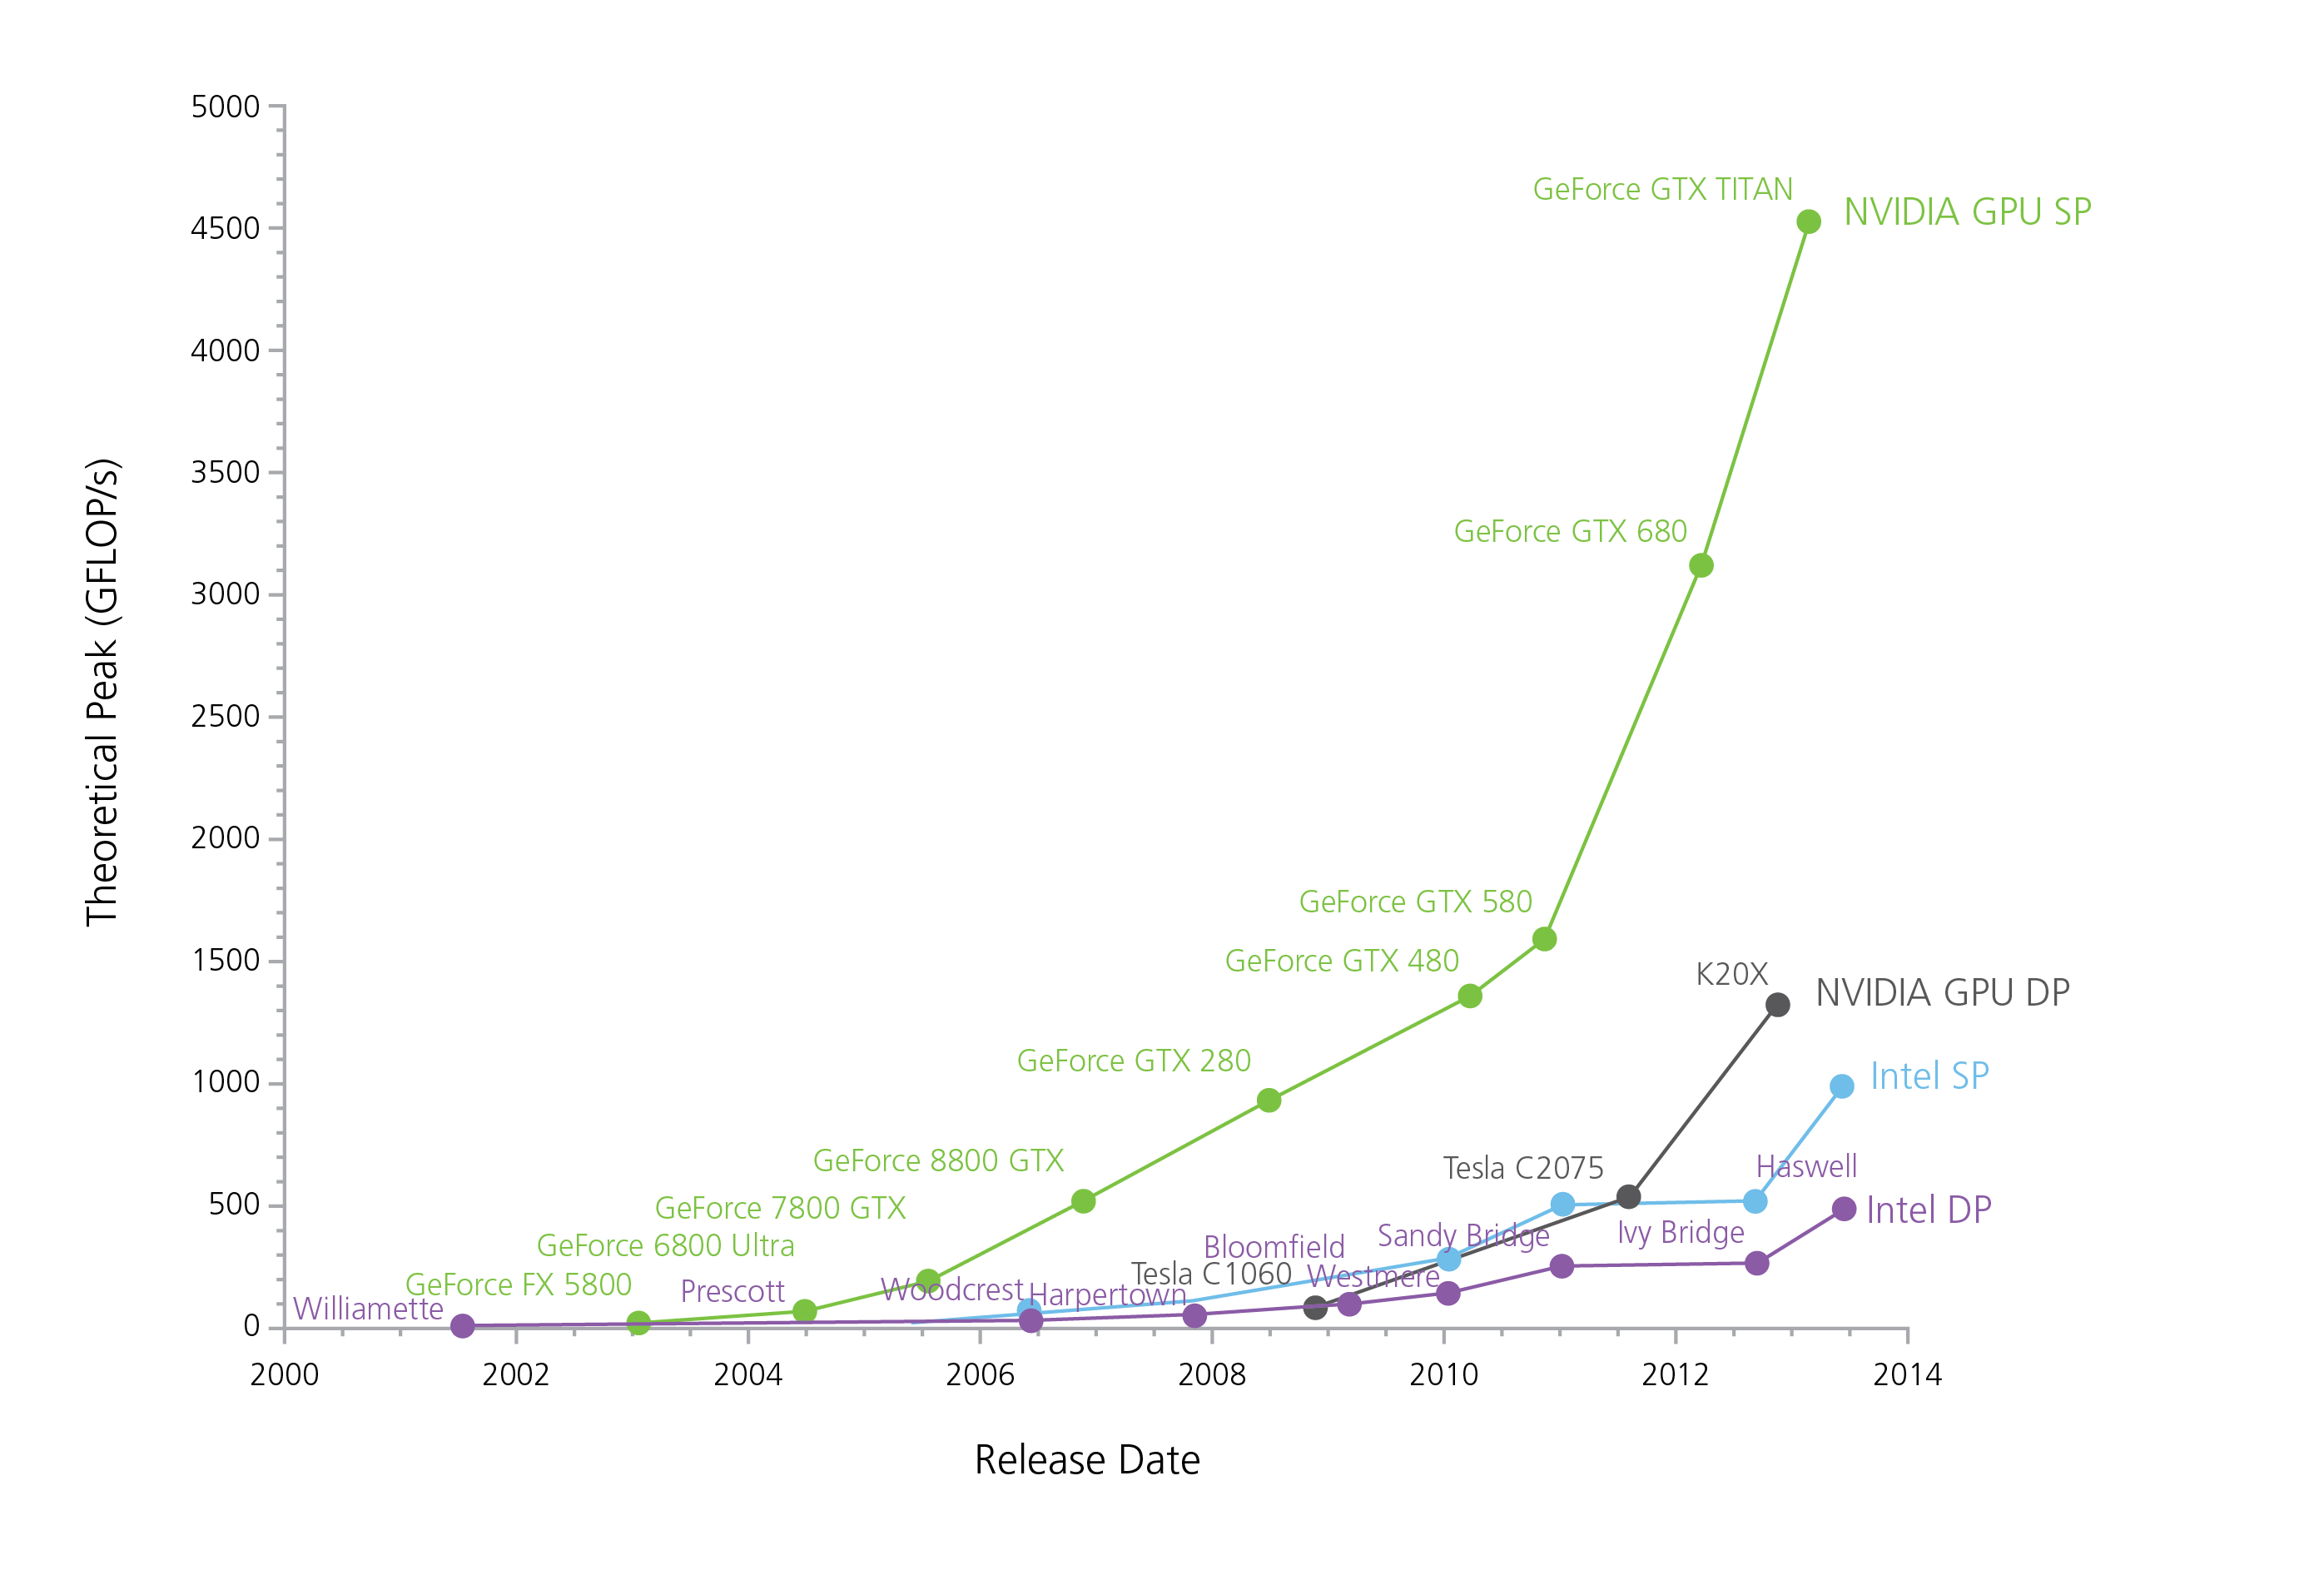
\includegraphics [width=0.9\textwidth]{Introduction/Figs/GPUstats.png}
    \caption{Performance comparison of GPU's over time. \\ \textbf{Source:} CPU vs. GPU Performance, MichaelGalloy.com}
    \label{fig:GPUStats}
\end{figure}

Higher level skeleton programming libraries have also been developed, which aims to make the parallelization of a problem easier with the use of higher-order functions, skeletons. One such library is SkePU, which was originally developed by Johan Enmyren and Christoph Kessler at Linköping University \cite{enmyren2010skepu}. The major revision SkePU 2 was designed by August Ernstsson, Lu Li and Christoph Kessler and is today maintained by August Ernstsson. Other alternatives exists such as \textbf{OpenAAC} which is a programming standard developed by Cray, CAPS, Nvidia and PGI \cite{OpenACC}, Nvidia's own template library for CUDA, \textbf{Thrust} \cite{Thrust}, and SYCL, which is is OpenCL's equivalent to Thrust \cite{SYCL}.


%********************************** %Second Section  *************************************
\section{Aim} %Section - 1.2

This paper aims to evaluate different GPGPU frameworks in terms of performance, portability, code complexity and features with less focus on the performance evaluation. A suitable benchmarking algorithm will be implemented in the GPGPU frameworks CUDA, OpenCL and DirectX direct compute, as well as an implementation in the higher level skeleton library SkePU. The parallelized implementations will be evaluated against a sequential implementation of the same problem.


%********************************** % Third Section  *************************************
\section{Research questions}  %Section - 1.3 

\begin{itemize}
    \item What is a suitable benchmarking algorithm?
    \item How does a parallel implementation of the algorithm compare to a sequential implementation?
    \item What framework-specific optimization's can be done for the implementation?
    \item How does the frameworks compare in terms of portability, code complexity and performance and features?
\end{itemize}


%********************************** % Fourth Section  *************************************
\section{Delimitations}
This section will present some delimitations for the implementation and evaluation.

The selected algorithm will only be implemented in the discussed frameworks:
\begin{itemize}
    \item CUDA
    \item OpenCL
    \item DirectCompute
\end{itemize}

\noindent aswell as an implementation in SkePU, running OpenCL, CUDA, OpenMP and a sequential backend \cite{enmyren2010skepu}. The selected algorithm will thus not be implemented in other GPGPU frameworks such as OpenGL's compute shader, or a parallel CPU based implementation, using e.g OpenMP or similar frameworks.

Even though other optimization algorithms exists for the N-Body problem, only the Barnes-Hut algorithm will be implemented in this work. The reason for this is because the thesis will not focus on evaluating the performance of the frameworks when running the selected algorithm, but on the comparison between frameworks in terms of portability, code complexity and features, which multiple optimization techniques implementations won't contribute to. Furthermore to give the implementation a fair comparison, the tree-structure used in Barnes-Hut will be a sequential implementation and will be performed on the host.

\section{Related work}
This section describes previous research on the subject, both in terms of performance comparisons, but also what previous work and research has been done in terms of the N-Body problem as well as comparisons between the discussed frameworks.


\subsection{Framework comparison}
In 2016 a similar master thesis was performed by T. Sörman where the frameworks CUDA, OpenCL, DirectCompute and OpenGL was compared as well as how the GPGPU implementations performed compared to an multithreaded implementation in OpenMP. \cite{Torbjorn}. Also performed at MindRoad AB, the thesis compares the different frameworks primarily in terms of performance, unlike this thesis which puts more focus on the portability, code complexity and features of the different frameworks. This work will also evaluate the skeleton programming framework SkePU which was not included in Sörmans research \cite{enmyren2010skepu}. 

The algorithm Sörman evaluated is a parallel implementation of the fast fourier fransform (FFT), and the result showed that the fastest framework, CUDA, was twice as fast as the slowest, OpenCL, and that the although older frameworks OpenGL and DirectX, are competitive with both CUDA and DirectX in terms of performance.

A lot of previous research has been abducted on the subject of comparing the performance between CUDA and OpenCL. K. Karimi et. al. performed an performance comparison between the two frameworks which showed similar results to Sörmans comparison \cite{karimi2010performance}. Although the performance gap was more subtle in Karimi. et. al. work, the result still showed that CUDA was faster than OpenCL. 

Another more comprehensive study between the two frameworks was abducted by J. Fang et. al. \cite{fang2011comprehensive}. The conducted study compares OpenCL and CUDA in terms of performance when a wide variety of benchmarking algorithms, such as graph traversal, reduction as well the N-Body problem and more, are executed in the two frameworks. Unlike the previously discussed comparisons, the result showed that under a fair comparison the performance difference between the two frameworks was very subtle. 

Another comparison study between CUDA, OpenCL and OpenGL, as well as a CPU multicore implementation that uses OpenMP has been made by R. S. Oliveira et. al. \cite{oliveira2011comparing}. The comparison was based of implementations of the Cardiac Monodomain Equations, and the results showed that the OpenGL approach was the fastest with a speedup of 446 compared to the multicore implementation for a solution of a non-linear system of ordinary differential equations (ODEs). CUDA was the fastest for a numerical solution of parabolic partial diffential equations (PDEs) with a speedup of 8. OpenCL was the slowest for solving the PDEs and as fast as CUDA for solving ODEs.


Although a lot of research comparing CUDA and OpenCL have been made, very little comparisons has been made comparing SkePU with other frameworks. C. Kessler et. al. performed a comparison between SkePU running various backends, to various other implementations: \cite{enmyren2010skepu}
\begin{itemize}
    \item \textbf{ls-seq-def:} The default sequential implementation in LibSolve
    \item \textbf{ls-seq-A:} A slightly optimized variant of ls-seq-def.
    \item \textbf{ls-shm-def:} The default shared memory implementation in LibSolve. It uses pthreads and were run with 8 threads, one for each core of the benchmarking computer.
    \item \textbf{ls-shm-A:} A slightly optimized variant of ls-shm-def. It also uses pthreads and were run with 8 threads.
    \item \textbf{skepu-CL:} SkePU port of ls-seq-def using OpenCL as backend and running on one Tesla C1060 GPU.
    \item \textbf{skepu-CL-multi:} SkePU port of ls-seq-def using OpenCL as backend and running on two Tesla C1060 GPU.
    \item \textbf{skepu-CU:} SkePU port of ls-seq-def using CUDA as backend and running on one Tesla C1060 GPU.
    \item \textbf{skepu-OMP:} SkePU port of ls-seq-def using OpenMP as backend and utilizing 8 threads. 
    \item \textbf{skepu-CPU:} SkePU port of ls-seq-def using the default CPU backend.
    \item \textbf{CU-hand:} A ”hand” implemented CUDA variant. It is similar to the SkePU ports however no SkePU code was utilized. Instead CUBLAS functions were used where applicable and some hand made kernels.

\end{itemize}
\noindent The result of this comparison can be seen in figure \ref{fig:SkepuComparisonODE}. 
C. Kessler et. al. paper also included a comparison between an implementation of a dot product, with SkePU running on different backends compared to CUBLAS, an NVidia CUDA implementation of a dot product calculation. As can be seen in figure \ref{fig:SkepuComparisonDOT}, the results showed that the performance of the SkePU CUDA version is very similar to that of the CUBLAS version.

\begin{figure}[!htbp]
    \centering
    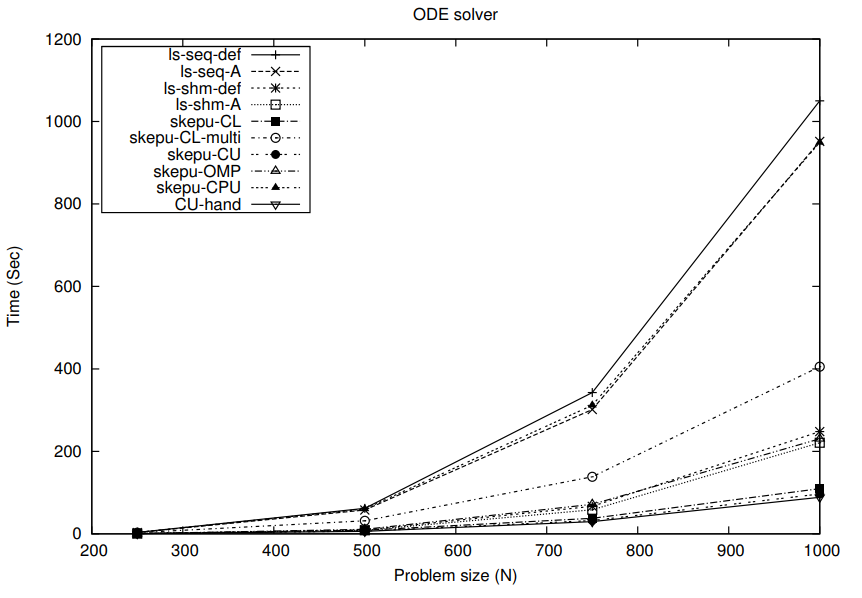
\includegraphics[width=\textwidth]{Introduction/Figs/SkePUComparison.png}
    \caption{SkePU times for running different LibSolve solvers for N =250,500,750 and 1000 with the BRUSS2D-MIX problem. \cite{enmyren2010skepu}}
    \label{fig:SkepuComparisonODE}
\end{figure}

\begin{figure}[!htbp]
    \centering
    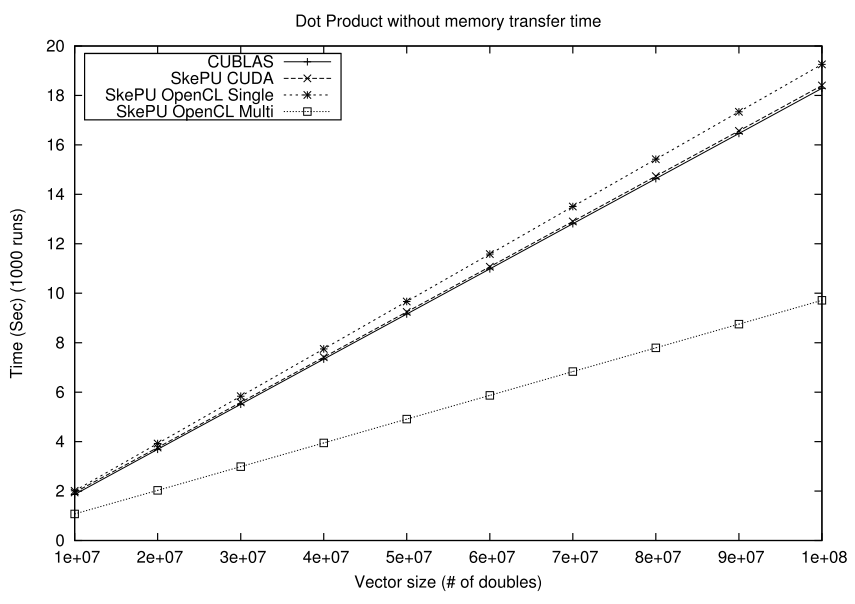
\includegraphics[width=\textwidth]{Introduction/Figs/SkePUComparisonDOT.png}
    \caption{Time for 1000 runs of dot product calculation without host-to-device memory transfer time. \cite{enmyren2010skepu}}
    \label{fig:SkepuComparisonDOT}
\end{figure}


\subsection{N-Body with Barnes-Hut}
The N-Body problem is a common implementation, and a lot of previous work has been done regarding the N-Body problem. In the book GPU Gems 3, L. Nyland et. al. at NVIDIA corporation describes an CUDA implementation of the N-Body used to generate an astrophysical simulation \cite{nyland2007fast}. The implementation is done in CUDA, and describes various methods how the CUDA implementation can be optimized with the use of e.g. shared memory, loop-unrolling and coalesced memory accesses. The result of the performance can be seen in figure \ref{fig:GPUGemsNBodyPerformance}. The implementation described in this article does not use the Barnes-Hut algorithm to further speed up the simulation, but instead use what Nyland et. al. call all-pairs, meaning that all N-bodies are compared to all other, resulting in the base implementation further described in section \ref{subsec:TheoryNBody}. 

\begin{figure}[!htpb]
    \centering
    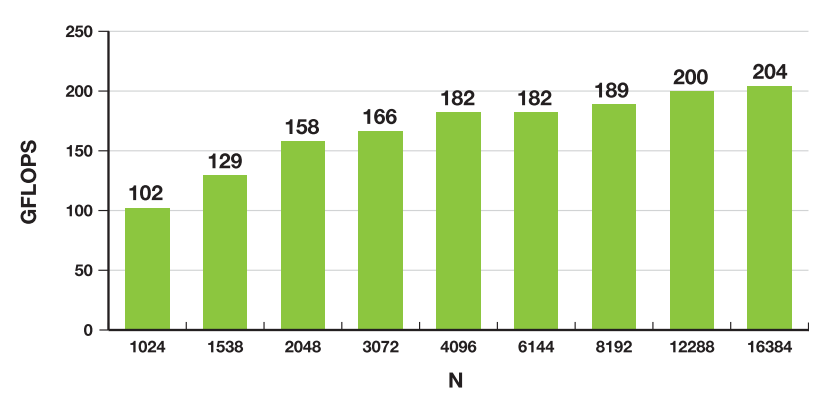
\includegraphics[width=\textwidth]{Introduction/Figs/GPUGemsNBodyComparison.png}
    \caption{N-Body performance increase as N grows. \cite{nyland2007fast}}
    \label{fig:GPUGemsNBodyPerformance}
\end{figure}

Another paper describing the N-body problem, and how it can be applied to astrophysical simulations is S. J. Aarseth's paper \cite{aarseth2003gravitational}. Aarseth's work describes the historical development of the N-body problem, as well as a detailed description of the physical properties of the N-Body problem.


M. Burtscher et. al. made an implementation of the N-Body problem in CUDA with the Barnes-Hut optimization \cite{burtscher2011efficient}. With focus on optimizing the implementation, most of the algorithm was performed on the GPU, resulting in minimal overhead of copying data back and forth between the host and device. M. Burtscher et. al. divided the implementation into six main steps, all performed on the GPU:
\begin{enumerate}
    \item Compute bounding box around all bodies
    \item Build hierarchical decomposition by inserting each body into octree
    \item Summarize body information in each internal octree node
    \item Approximately sort the bodies by spatial distance
    \item Compute forces acting on each body with help of octree
    \item Update body positions and velocities
\end{enumerate}

\noindent The implementation was only done in CUDA and the paper focuses how the implementation is optimized by e.g maximizing coalescing, minimize GPU/CPU data transfer, loop-unrolling etc. The resulting performance of the simulation when run in a sequential CPU implementation, all-pairs parallel implementation as well as a parallel Barnes-Hut implementation can be seen in figure \ref{fig:BurtscherResults}.

\begin{figure}[!htpb]
    \centering
    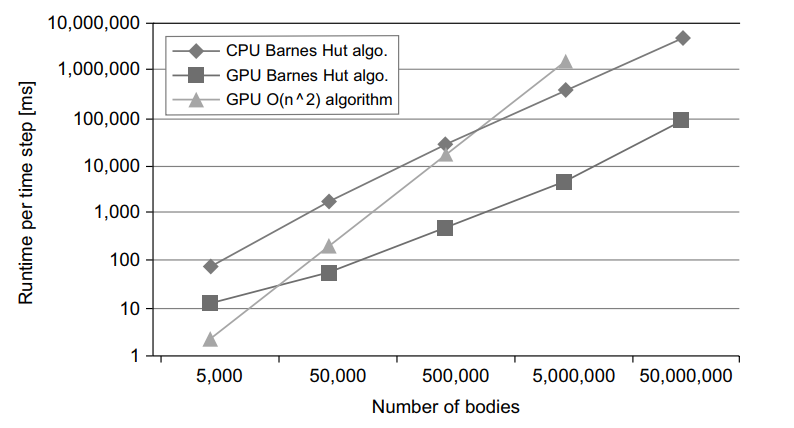
\includegraphics[width=\textwidth]{Introduction/Figs/CPUvsGPUn2vsBarnesHut.png}
    \caption{Runtime per simulated step in M. Burtscher et. al. CUDA implementation of the N-Body problem. \cite{burtscher2011efficient}}
    \label{fig:BurtscherResults}
\end{figure}

\nomenclature[z-ODE]{ODE}{Ordinary Differential Equations}
\nomenclature[z-PDE]{PDE}{Partial Differential Equations}
\nomenclature[z-FFT]{FFT}{Fast Fourier Transform}
\nomenclature[z-OPC]{OpenCL}{Open Computing Language}
\nomenclature[z-CPU]{CPU}{Central Processing Unit}
\nomenclature[z-GPU]{GPU}{Graphics Processing Units}
\nomenclature[z-GPG]{GPGPU}{General-purpose Computing on Graphics Processing Units}
\nomenclature[z-ILP]{ILP}{Instruction Level Parallelism}
%!TEX root = ../thesis.tex

\chapter{Theory}
This chapter describe background theory about parallelism, and why it has become a highly relevant topic in modern system architectures. It also describes the different frameworks and libraries evaluated in this work, as well as some typical parallelizable problems. Finally, benchmarking algorithms are presented and a motivation why each algorithm is suitable for this kind of evaluation.

\section{Background} 
As mentioned in section \ref{sec:IntroductionMotivation}, the performance inclination of single-cored CPU's has reached a limit. The reason for this decline is due to three walls.

The \textbf{ILP-wall} which states that there is not enough instruction level parallelism to keep the CPU busy. Some techniques do however exist such as Very Large Instruction Word (VLIW) and the Superscalar Architecture but they are limited by the hardware complexity.

The second wall, the \textbf{Memory wall} is reached because of the gap between the CPU speed and accesses to off-chip memory.

As mentioned in section \ref{sec:IntroductionMotivation} and visualized in figure \ref{fig:CPUstats}, Moore's law is still valid, but the increased amount of on-chip micro transistors needs an increased amount of power, which leads to overheating problems and has been named the \textbf{Power wall}.

The solution to all of these problems are however the same. Although it is not possible to increase the single-thread performance, we can put more cores on a chip. Today, all major CPU manufacturers develop multi-core CPU's, and most devices used in our everyday life such as smartphones, laptops 
and desktop CPU's have a multi-core architecture, and the number of cores on a chip seems to be increasing, see figure \ref{fig:CPUstats}

\begin{figure}[!h]
    \centering
    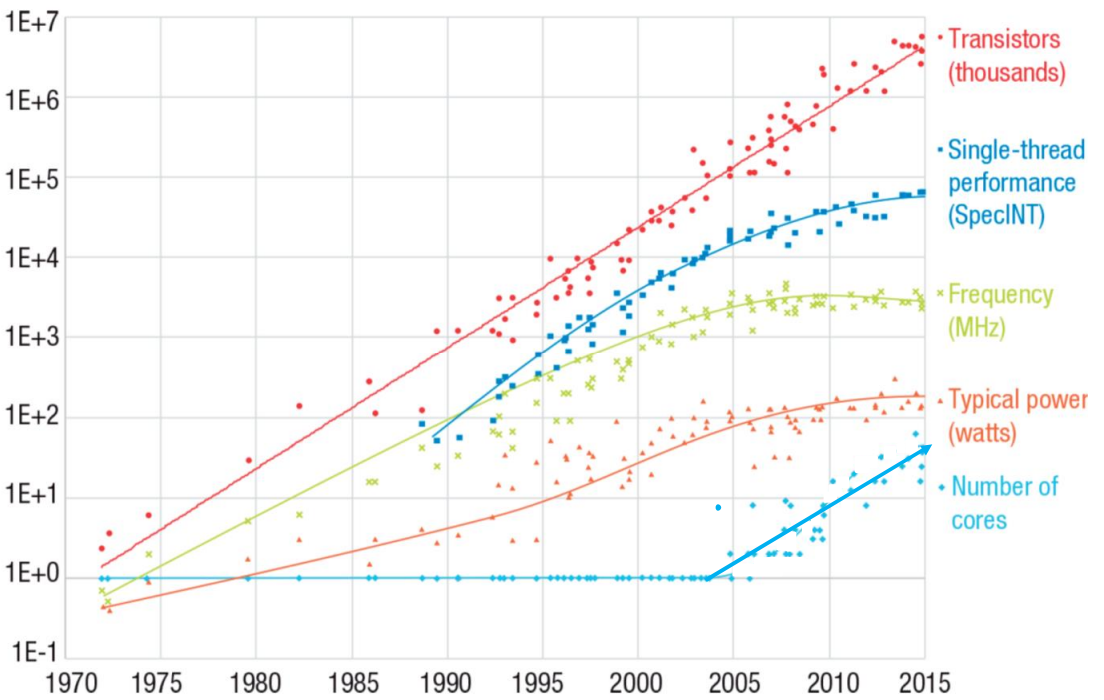
\includegraphics[width=0.8\textwidth]{Introduction/Figs/CPUStats.png}
    \caption{Development of CPU's. \cite{CPUStats}}
    \label{fig:CPUstats}
\end{figure}

The idea of putting multiple cores on a single chip which may be run in parallel is not new technology, GPU's has long been using this architecture and modern GPU chips contains hundreds of cores. This massive amount of parallelism and parallel computing power are designed to render graphics on screen and perform fast algebraic calculations commonly used in computer graphics such as matrix or vector operations, and is thus parallel in nature. But it can also be used for more general purpose computing, as quoted by Thompson et. al. "...Most of this time, however, this power is going unused because it is only
being exploited by graphics applications" \cite{thompson2002gpgpu}.


\subsection{GPGPU History}
With the release of programmable shaders and floating point precision GPU's in 2001, the idea of performing general purpose computing on the GPU became popular. Early research on the subject implemented simple, well-parallelizable problems such as vector or matrix additions, and one of the first scientific GPGPU problems that outperformed the CPU was a implementation of LU factorization. \cite{CUDAtoOpenCL}. Another research on the subject performed by Thompson et. al. from 2002 showed that a simple arithmetic operation applied to all elements of a vector of varying sized, outperformed the CPU once the problem size grew large enough which is generally the case for GPGPU.\cite{thompson2002gpgpu}.

These early adaptations of GPGPU used the traditional rendering pipeline by performing computations in the fragment/pixel shaders of the application, using the two major application programming interfaces (API) OpenGL and DirectX. Although this approach adds some limitations, it is still quite widespread and are still in use today. Since then, both OpenGL and DirectX has released shaders specifically purposed for GPGPU. These types of shaders are known as Compute Shaders (CS), and Microsoft released their CS support with the DirectCompute as a part of the DirectX collection of APIs.

Later on Nvidia realized the potential of GPGPU and developed the CUDA framework to make GPGPU programming easier by adding lots of features and simplifying the data transfer. Later on, OpenCL was released with the same purpose, with a lot of backing major companies such as Apple and IBM. It is today maintained by the Khronos group, which also maintains OpenGL.

\section{GPU} \label{sec:GPUTheory}
As previously discussed in section \ref{sec:IntroductionMotivation}, whilst a CPU may have a few cores (~8 cores on a modern desktop machine) that can be run in parallel, modern GPUs have hundreds of cores. Although not as powerful as a single CPU core, this extensive amount of cores allows for massively parallel computation to be made. Moreover, the GPU allows for a much higher theoretical bandwidth than a CPU as is illustrated in figure \ref{fig:GPUGFLOPS}.

\begin{figure}[!htpb]
    \centering
    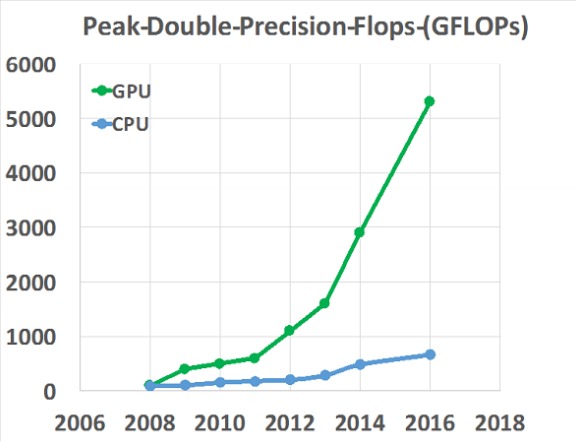
\includegraphics[width=0.6\textwidth]{Theory/Figs/GFLOPSGPU.png}
    \caption{Theoretical giga floating point operations per second (GFLOPS) performance of CPUs versus GPUs. \cite{Ingemar9b}}
    \label{fig:GPUGFLOPS}
\end{figure}
\nomenclature[z-GFLOPS]{GFLOPS}{Giga Floating Point Operations Per Second}

\noindent This is due to the efficient area use of the GPU architecture as visualized in figure \ref{fig:GPUvsCPUArchitecture}, but in particular the SIMD architecture (Single Instruction, Multiple Data). SIMD simplifies the instruction handling since all cores receive the same instruction which is applied to multiple data in parallel, usually stored in list structures such as arrays. The instruction that should be applied to each data-element is written as a separate piece of code, separated from the main program and run on the device (GPU, FPGA or other parallel hardware). Different frameworks use different languages in which this code is implemented, but the general GPGPU term used for this is a kernel. The most common way of executing a kernel is done in the following steps:
\nomenclature[z-SIMD]{SIMD}{Single Instruction, Multiple Data}
\begin{enumerate}
    \item Allocate memory from the host (typically CPU) to the device (GPU or other parallel hardware).
    \item Copy data from the host to the allocated memory on the device.
    \item Launch the kernel, executing on the data that was just copied.
    \item Copy back the result from the device to the host.
\end{enumerate}

\begin{figure}[!h]
    \centering
    \begin{subfigure}[b]{0.4\textwidth}
        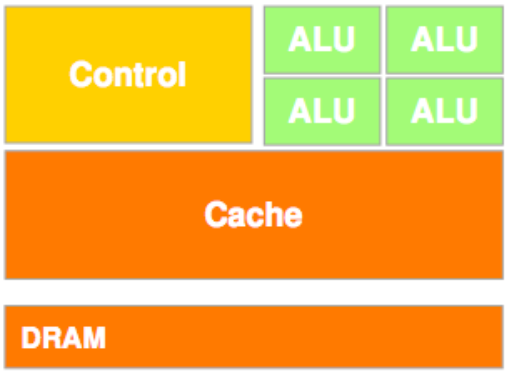
\includegraphics[width=\textwidth]{Theory/Figs/CPUArch.png}
        \caption{}
    \end{subfigure}
    ~ 
    \begin{subfigure}[b]{0.4\textwidth}
        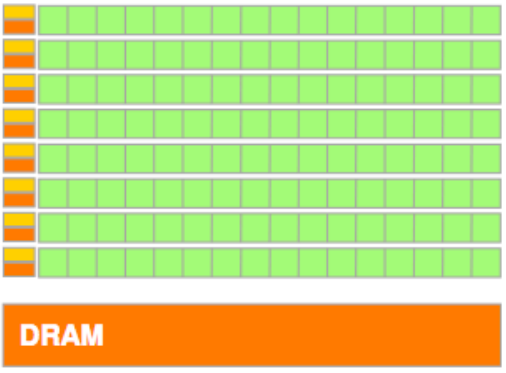
\includegraphics[width=\textwidth]{Theory/Figs/GPUArch.png}
        \caption{}
    \end{subfigure}
    \caption{Area use of CPU (a) and GPU (b)}
    \label{fig:GPUvsCPUArchitecture}
\end{figure}



\section{Frameworks}
This section briefly describes the different frameworks and APIs that are a subject of comparison in this comparative study. Each section contains sample code of a very simple vector addition kernel for the respective frameworks. The popularity of the frameworks is based upon the chart in figure \ref{fig:GoogleTrendsPopularity} from Google Trends.

\subsection{CUDA}
Released in 2007, CUDA developed by Nvidia was the first major GPGPU framework to be released. It aims to make the parallelization of a problem more manageable by providing an easy to work with API. One downside of CUDA is that is has a weak portability and can only be run on Nvidia GPU's. Despite this limitation it is a very popular framework among GPGPU developers, see figure \ref{fig:GoogleTrendsPopularity} \cite{AboutCuda}.  The installation procedure is very simple, all that is needed is a CUDA development toolkit which can be downloaded from Nvidia's webpage.

CUDA is an extension of the C/C++ language, allowing the developer to write both device and host code in a C/C++ like fashion. To run and compile CUDA, a custom compiler is used, NVCC. To define what parts of the code that should be run on the host and the device the keywords \lstinline{__host__} and \lstinline{__device__} is used, although the \lstinline{__host__} keyword is rarely seen since it is specified per default. To specify that the next block of code is a kernel the keyword \lstinline{__global__} is used.
Each thread in a CUDA program is organized in a block, which in turn is organized in a grid, see figure \ref{fig:CUDAGridBlockThreads}. When launching a kernel, arguments specifying the grid and block-dimension must be supplied. There exists a few different types of memory in CUDA, these memory types are listed in table \ref{tab:CUDAMemoryTypes} 

A very simple CUDA kernel that performs a vector addition can be seen in Listing \ref{lst:cudaVectorAdd}.

\begin{table}

    \begin{tabularx}{\textwidth}{ |X|X|X|X|X| }
      \hline
      \rowcolor{gray}
      \textbf{Memory} &  \textbf{Location} &  \textbf{Cached} &    \textbf{Access} &    \textbf{Scope} \\ \hline 
      \textbf{Register} & On-chip   & Cached    & Access        & Thread \\ \hline 
      \textbf{Local}    & Off-chip  & No        & Read/write    & Thread \\ \hline 
      \textbf{Shared}   & On-chip   & No        & Read/write    & Block \\ \hline 
      \textbf{Global}   & Off-chip  & N/A       & Read/write    & Global + host \\ \hline 
      \textbf{Constant} & Off-chip  & Yes       & Read          & Global + host \\ \hline 
      \textbf{Texture}  & Off-chip  & Yes       & Read          & Global + host \\ \hline 
    \end{tabularx}

\caption{\label{tab:CUDAMemoryTypes} CUDA memory types.}
\end{table}

\begin{figure}[!htpb]
    \centering
    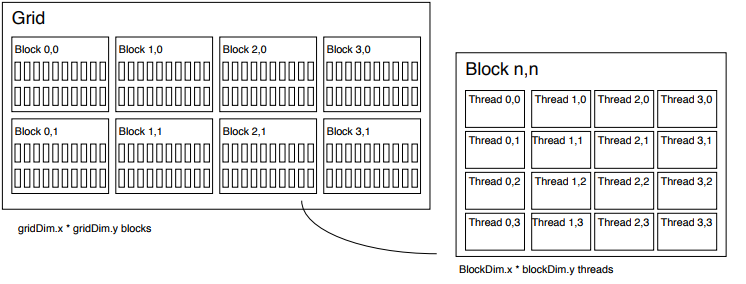
\includegraphics[width=\textwidth]{Theory/Figs/CUDAGridBlockThreads.png}
    \caption{Hierarchical CUDA model for grids, blocks and threads.}
    \label{fig:CUDAGridBlockThreads}
\end{figure}

\begin{lstlisting}[caption={CUDA vector addition kernel}, label={lst:cudaVectorAdd}, frame=single] 
__global__ void add(int *out, const int *in_a, const int *in_b)
{
	int idx = blockDim.x * blockIdx.x + threadIdx.x;
	if (idx < SIZE)
		out[idx] = in_a[idx] + in_b[idx];
}
\end{lstlisting}



\subsection{OpenCL} \label{sec:OpenCLTheory}
For a couple of years, CUDA was the only framework developed for the sole purpose of GPGPU and Nvidia had no competitors on the GPGPU front. That is until Apple took the initiative to develop a competitor, and backed by a lot of major companies, OpenCL was developed. OpenCL sought to offer a more portable and wide variety of parallel devices, and OpenCL offers the ability to run parallel implementations on other devices than just GPU's such as FPGA's and ARM devices. OpenCL is an open standard, and implementations are available from Apple, AMD, Intel, Nvidia and more \cite{KhronosOpenCL}. Because of this, the portability of OpenCL is good, and it can be run on most systems, provided a parallel hardware is present. Since there are multiple implementations of OpenCL, the setup procedure differs, but OpenCL is usually provided by the manufacturers drivers.

The syntax in OpenCL is quite similar to that of CUDA although some differences exist. Although the hierarchy model is very similar, OpenCL uses different terms for these, as well as the memory types. These are listed in table \ref{tab:OpenCLvsCUDA}. Similar to CUDA, OpenCL uses keywords, the keyword that specifies a kernel is \lstinline{__kernel}. Data that resides in the global and local memory are specified using the \lstinline{__global} and \lstinline{__local} keywords.
Whilst CUDA automatically selects a device of the available hardware on the system, OpenCL needs to know what device to run on. Thus the setup procedure differs slightly from the procedure described in section \ref{sec:GPUTheory}. Before copying data and executing the kernel, a OpenCL program first have to do the following steps before doing the steps described in \ref{sec:GPUTheory}:

\begin{enumerate}
    \item Get a list of platforms
    \item Choose a platform
    \item Get a list of devices
    \item Choose a device
    \item Create a context
    \item Load and compile kernel code    
\end{enumerate}

A simple kernel that does the same thing as the CUDA kernel described in listing \ref{lst:cudaVectorAdd}, that is perform a vector addition on two vectors, are given in listing \ref{lst:OpenCLVectorAdd}.

\begin{lstlisting}[caption={OpenCL vector addition kernel}, label={lst:OpenCLVectorAdd}, frame=single] 
__kernel void vectorAddition(__global read_only int* vector1, 
                                __global read_only int* vector2, 
                                __global write_only int* vector3)
{
	int indx = get_global_id(0);
	vector3[indx] = vector1[indx] + vector2[indx];
}
\end{lstlisting}

\begin{table}[!h]
    \begin{tabularx}{\textwidth}{ |X|X| }
      \hline
      \rowcolor{gray}
      \textbf{OpenCL}   &  \textbf{CUDA} \\ \hline 
        Compute Unit    & Multiprocessor (SM) \\ \hline
        Work item       & Thread \\ \hline
        Work group      & Block \\ \hline
        Local memory    & Shared memory \\ \hline
        Private memory  & Registers \\ \hline
    \end{tabularx}
\caption{\label{tab:OpenCLvsCUDA} CUDA vs OpenCL terms}
\end{table}




\subsection{DirectCompute}
Initially released with the DirectX 11 API, DirectCompute is Microsoft's technology for GPGPU, and unlike CUDA or OpenCL which relies on launching kernels, DirectCompute runs a CS as a part of the graphics pipeline. Although released with the DirectX 11 API, DirectCompute runs on GPUs that use either DirectX 10 or 11 \cite{NVidiaDirectCompute}. Since DirectCompute is a part of the DirectX API, no additional setup is required, but DirectCompute can only be run on Windows PCs that have a support DirectX version.

Since DirectCompute is not a framework, but a API of the DirectX suite and uses the concept of CS to perform GPGPU calculations, it is quite different from CUDA or OpenCL. All of the computing in DirectCompute is done on a CS, which would be the equivalent to a kernel in CUDA or OpenCL. The setup process is quite similar to the one described in section \ref{sec:GPUTheory}, but uses the traditional graphics way of copying data between the host and the device using buffers, which are copied to the CS before the CS is run. The CS is written in the high-level shading language (HLSL) also developed by Microsoft, and a simple CS that performs a vector addition (using a structured buffer) can be seen in listing \ref{lst:DirectComputeVectorAdd}.

\begin{lstlisting}[caption={DirectCompute vector addition CS}, label={lst:DirectComputeVectorAdd}, frame=single] 
struct BufType
{
    int i;
    float f; 
};

StructuredBuffer<BufType> Buffer0 : register(t0);
StructuredBuffer<BufType> Buffer1 : register(t1);
RWStructuredBuffer<BufType> BufferOut : register(u0);

[numthreads(1, 1, 1)]
void CSMain( uint3 DTid : SV_DispatchThreadID )
{
    BufferOut[DTid.x].i = Buffer0[DTid.x].i + Buffer1[DTid.x].i;
    BufferOut[DTid.x].f = Buffer0[DTid.x].f + Buffer1[DTid.x].f;
}

\end{lstlisting}



\subsection{SkePU 2}
SkePU is a high-level skeleton programming framework originally developed by Johan Enmyren and Christoph W. Kessler at Linköping University \cite{enmyren2010skepu}. The framework aims to simplify the parallelization of a implementation by using skeleton functions such as map and reduce which are common parallel algorithms, which makes SkePU very different from the previously mentioned frameworks. When using SkePU, the developer specifies what backend the implementation should run. The currently available backends are sequential C, OpenMP, OpenCL, CUDA, and multi-GPU OpenCL and CUDA \cite{LiUSkePU}. The major revision SkePU 2 was designed by August Ernstsson, Lu Li and Christoph Kessler and is today maintained by August Ernstsson. Further mentions of SkePU will refer to SkePU 2.

Since SkePU is not a GPGPU framework, but a skeleton framework, it is different from the previously discussed CUDA, OpenCL and DirectCompute in terms that it don't involves writing a kernel. Although the setup procedure is quite complicated, once installed it is very portable since it is able to run with most GPU's, depending on the selected backend. As presented in the previous sections, a SkePU vector addition program using the Map-skeleton is supplied in listing \ref{lst:SkePUVectorAdd}

\begin{lstlisting}[caption={SkePU vector addition}, label={lst:SkePUVectorAdd}, frame=single] 

float add(float a, float b){
	return a + b;
}

int main(){
    /**
    ...
    **/
    
    auto addition = skepu2::Map<2>(add);
    
    skepu2::Vector<float> v1(N, 1.0f), v2(N, 2.0f), res(size, 3.0f);
    addition(res, v1, v2);
}



\end{lstlisting}

\begin{figure}[!htbp]
    \centering
    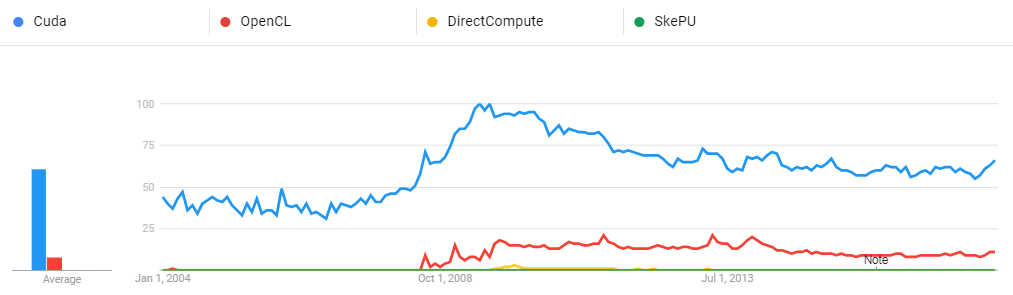
\includegraphics[width=\textwidth]{Theory/Figs/GoogleTrendsComparison.png}
    \caption{Popularity over time of CUDA, OpenCL, DirectCompute and SkePU. Numbers represent search interest relative to the highest point on the chart for the given region and time. \ \textbf{Source:} Google trends}
    \label{fig:GoogleTrendsPopularity}
\end{figure}



\section{Algorithm evaluation}
In this section, algorithms that are suitable for a benchmarking application is briefly explained and discussed. The discussed algorithms are compared, and a motivation of the selected algorithm are given which is explained and discussed further in section \ref{sec:TheoryNBody}.

\subsection{Parallel QuickSort}
As a popular sequential sorting algorithm, the QuickSort algorithm invented by C.A.R  Hoare, is a recursive divide-and-conquer based sorting algorithm \cite{hoare1962quicksort}. The algorithm has a time complexity of $O(n \ log \ n)$ in the best case, a worst case complexity of $O(n^2)$, and an average run time of $O(n \ log \ n)$. A pivot element $A[q]$ is selected from the array to be sorted. The array is then partitioned into two subarrays $A[p...q-1]$ such that all elements are less than $A[q]$, and $A[q+1...r]$ such that all elements are greater than or equal to $A[q]$. After this partitioning step, the pivot are in its correct step. This procedure are then applied recursively to the subarrays until the entire array is sorted. Pseudocode for the algorithm can be seen in Algorithm \ref{alg:quicksort}. The comparison part of the algorithm is well suited for a parallel implementation, but due to the data dependency of the algorithm, parallelizing the partitioning stage is a more difficult task. Some implementations and papers describng how the algorithm can be parallelized do however exist \cite{cederman2009gpu}\cite{sanders1997efficient}\cite{chen2009fast}.

\begin{algorithm}
    \caption{Quicksort pseudocode}
    \label{alg:quicksort}
    \begin{algorithmic}[1]
        \Procedure{quicksort}{$A, lo, hi$}
            \If{$lo < hi$}
                \State $p:=$ \Call{partition}{$A, lo, hi$}
            	\State \Call{$quicksort$}{$A, lo, p-1$}
            	\State \Call{$quicksort$}{$A, p+1, hi$}
            \EndIf
        \EndProcedure
        
        \Procedure{partition}{$A, lo, hi$}
            \State $pivot := A[hi]$
            \State $i := lo - 1$
            \For{$j := lo$ \textbf{to} $hi-1$}
                \If{$A[j] < pivot$}
                    \State $i := i + 1$
                    \State \Call{$swap$}{$A[i],A[j]$}
                \EndIf
            \EndFor
            \If{$A[hi] < A[i + 1]$}
                \State \Call{$swap$}{$A[i + 1],A[hi]$}
            \EndIf
        \EndProcedure
    \end{algorithmic}
\end{algorithm}

A parallel implementation of the Quicksort algorithm would be an interesting algorithm to use for a benchmark application of this degree. The performance of an parallel implementation could be compared to the classical sequential QuickSort algorithm for varying problem sizes, although due of the triviality of the implementation this algorithm was discarded.

\subsection{Distance transform}
First presented by C.Green of Valve Softworks, a method which allows improved rendering of glyphs composed of curved and linear elements was proposed \cite{green2007improved}. The technique works by generating a distance transform (DT) from a high-resolution texture by measuring the distance between a background texel to the closest foreground texel. The distance field is then stored into a channel of a lower-resolution texture, resulting in a texture with a arbitrary resolution, whilst occupying a small amount of video random access memory (VRAM). This low-resolution texture can then be rendered by using alpha-testing and alpha-thresholding features of modern GPU's with great results as illustrated in figure \ref{fig:GreensDT}. 

\begin{figure}[!h]
    \centering
    \begin{subfigure}[b]{0.27\textwidth}
        
\includegraphics[width=\textwidth]{Theory/Figs/ValveAlphaBlended.png}
        \caption{Alpha-blended}
        \label{fig:valveA}
    \end{subfigure}
    ~
    \begin{subfigure}[b]{0.3\textwidth}
        
\includegraphics[width=\textwidth]{Theory/Figs/ValveAlphaTested.png}
        \caption{Alpha tested}
        \label{fig:valveA}
    \end{subfigure}
    ~ 
    \begin{subfigure}[b]{0.3\textwidth}
        
\includegraphics[width=\textwidth]{Theory/Figs/ValveGreensTechnique.png}
        \caption{Green's technique}
        \label{fig:valveC}
    \end{subfigure}
    \caption{Vector art encoded in a 64x64 texture using (a) simple bilinear filtering (b) alpha testing and (c) Green's distance field technique}
    \label{fig:GreensDT}
\end{figure}

S. Gustavson et. al. later proposed an improved version of Green's technique, using the Euclidean distance to generate a DT \cite{gustavson2011anti}. Whilst Green's description of the proposed algorithm was quite sparse, Gustavson et. al. technique described the general implementation more detailed. Although the general technique described by Green and Gustavson et. al. only describe the two dimensional case, the distance transform has also been extended to three dimensions \cite{jones20063d}. 

One of the problems with the discussed distance transform is the ability to produce sharp features such as corners, and solutions to this problem has not been further investigated. Since the technique works on pixel/voxel level, the algorithm is well parallelizable, and an idea to further investigate this discussed problem was presented. This would however drift apart from the main idea of this research and was thus discarded.

\subsection{N-Body} \label{subsec:TheoryNBody}

The final proposed algorithm is the N-Body problem. Although the base implementation of the algorithm is fairly trivial and embarrassingly parallel, the algorithm can be further optimized by using the Barnes-Hut algorithm, reducing the time complexity from $O(n^2)$ to $O(n \ log \ n)$ \cite{barnes1986hierarchical}.  The N-Body problem as well as the Barnes-Hut algorithm is further described in section \ref{sec:NBodyTheory}.

\subsection{Choice of algorithm}

The choice of algorithm to be implemented and used to evaluate the different frameworks in this work was motivated to be complex enough so that a fair comparison between the frameworks could be made. If the algorithm was too trivial or embarrassingly parallel, the risk would be that framework specific features could be less utilized, and it would be difficult to compare the frameworks in this aspect. It would also raise the risk where the framework-part of the implementation is to small for a fair comparison to be made. 

With this in mind, the algorithm had to be complex enough so that a fair comparison could be made, but not to complex so that the algorithm couldn't be implemented in the given amount of time. Another motivation of the choice of algorithm was that it would include more complex data structures, and not just lists like arrays or vectors. 

The algorithm that best suits this motivation is the N-Body problem when optimized using the Barnes-Hut algorithm. Although the base case of the algorithm is embarrassingly parallel and fairly trivial to implement in any of the discussed frameworks, when optimized using the Barnes-Hut algorithm it gets more complex. The implementation must be able to handle the creation and traversal of trees which is not a very common implementation in GPGPU applications.

\section{N-Body} \label{sec:NBodyTheory}
The following section will describe the theory behind N-Body problem. A description of base problem is presented, followed by a description of the Barnes-Hut algorithm, and how it can be applied to the N-Body simulation to improve the performance.

\subsection{Base problem}
An N-body simulation is a numerical approximation of the behaviour of bodies in a system. A common implementation of the N-Body problem is a astrophysical simulation where each body represents a celestial body such as a star, galaxy or planet. Other astrophysical applications of the N-body problem can be used on a smaller scale to simulate a e.g. 3-body simulation of the earth, moon and sun. The simulation approximates how the celestial bodies behave over time when each body is affected by gravitational forces from all the others. It has also been used in physical cosmology, where N-Body simulations have been used to study the formation of e.g. galaxy filaments and galaxy halos from the influence of dark matter. \cite{navarro1996structure}

The N-body problem has also been used in Plasma physics, where the bodies are ions or electrons, and in molecular dynamics where the bodies represent molecules or atoms (usually in fluid state). In fluid dynamics the vortex blob method for solving Navier-Stokes equations, and boundary value problems have been solved rapidly by using N-Body methods. \cite{greengard1988rapid}

Another application where the N-Body simulation are known to be used is protein folding, where N-body simulations are used to calculate electrostatic and van der
Waals forces. It is also used in the computer graphics field, where it is used for turbulent fluid flow simulation and global illumination computation. \cite{nyland2007fast}.

The simulation made in this work is a astrophysical simulation of a cluster of stars, where each star is affected by gravitational forces from all others. As mentioned earlier this is one of the most common applications of N-Body problem and many papers and implementations regarding this kind of simulation has been made earlier \cite{aarseth2003gravitational}\cite{burtscher2011efficient}\cite{nyland2007fast}. 

\subsubsection{General formulation}
Consider $n$ point masses $m_i$ where $i \in [1, 2,..., n]$. Each point mass has a position vector $p_i$ in two or three dimensional space $\mathbb{R}^3$. 
Newton's second law states that mass times acceleration $m_i \frac{d^2 \boldsymbol p_i}{dt^2}$ is equal to the sum of all of the forces applied on the mass. In a astrophysical simulation, the only force applied to a body is the gravitational force, and Newtons law of gravity says that the gravitational force applied to a mass $m_i$ by a mass $m_j$ is given by the equation
\begin{equation}
    F_{ij} = \frac{G m_i m_j (\boldsymbol p_j - \boldsymbol p_i)}{|| \boldsymbol p_j - \boldsymbol p_i|| ^3}
\end{equation}
\noindent where $G$ is the gravitational constant and $|| \boldsymbol q_i - \boldsymbol q_j||$ is the magnitude of the distance between the masses. Summing over all masses, the total gravitational force $F_i$ applied to mass $m_i$ results in the n-body equations of motion:
 
\begin{equation} \label{eq:totGravForce}
    F_i = m_i\frac{d^2 \boldsymbol p_i}{dt^2} = \sum_{j=1, j\neq i}^n \frac{G m_i m_j (\boldsymbol p_j - \boldsymbol p_i)}{|| \boldsymbol p_j - \boldsymbol p_i|| ^3}
\end{equation}

Equation \ref{eq:totGravForce} has be be applied to each point mass $m_i$ in each timestep of the simulation, and thus have to be compared to all other $n-1$ point masses in the system resulting in a time complexity of $O(n^2)$. Pseudo-code of this \textit{all-pairs} n-body calculation using equation \ref{eq:totGravForce} can be seen in algorithm \ref{alg:allpairspseudocode}. By analyzing equation \ref{eq:totGravForce} and the pseudocode given in \ref{alg:allpairspseudocode}, we can conclude that there are two parts of the algorithm that can be parallelized. Using $p=n$ processors, the outer for-loop in the main procedure can be parallelized, resulting in each particles body-body interaction is calculated by a single process. Once the particles velocities have been updated, the position updating is embarrassingly parallel using a suitable integration scheme, e.g Runge-Kutta or Euler integration.

\begin{algorithm}
    \caption{All pars N-body pseudocode}
    \label{alg:allpairspseudocode}
    \begin{algorithmic}[1]

    \Procedure{BodyForce}{$p_i, p_j$}
        \State $F_i := 0$
        \State $Gm_im_j := G *p_i.m * p_j.m$
        \State $dPos := p_i - p_j$
        \State $distance := dist(dPos)$
        \State $magn3 := abs(dist)^3$
        \State $F_i := Gm_im_j * dPos / magn3$
        \State \Return $F_i$
        
    \EndProcedure
    
    \Procedure{main}{}
    
        \Comment{Update velocities}
        \For{$i:=0$ \textbf{to} $n$}
            \State $p_i := particles[i]$
            \State $F_i := {0,0,0}$
            \For{$j:=0, j\neq i$ \textbf{to} $n$}
                \State $p_j := particles[j]$
                \State $F_i := F_i +$ \Call{$BodyForce$}{$p_i, p_j$}
            \EndFor
            \State \textbf{od} % Inner for loop
            \State $p[i].v = p[i].v + dt*F_i$
        \EndFor
        \State \textbf{od} % Outer for loop
        
        \Comment{Update positions}
        \For{$i:=0$ \textbf{to} $n$}
            \State $p_i := particles[i]$
            \State $p_i.pos = p_i.pos + p_i.v * dt$
        \EndFor
        \State \textbf{od}
    \EndProcedure
        
        
    \end{algorithmic}
\end{algorithm}

Although this all-pairs implementation is straightforward and could be implemented effortlessly, with the time complexity $O(n^2)$ it is not very performance efficient. Various methods to improve the performance of the algorithm has been investigated by using hierarchical methods such as fast multipole method (FMM), the Barnes-Hut algorithm and a radiosity method. \cite{singh1995load}\cite{barnes1986hierarchical} 

Both Barnes-Hut, further discussed in section \ref{subsec:BarnesHut}, and the FMM uses a recursive decomposition of the computational domain into a tree structure. The FMM is very similar to the Barnes-Hut method. The main difference between FMM and Barnes-Hut is that while the Barnes-Hut only computes particle-particle, or particle-cell interactions, the FMM also computes interactions between internal cells directly. Due to the FMM method beeing more complex implementation wise, only the Barnes-Hut algorithm is implemented in this work \cite{singh1995load}. The radiosity implementation is mostly used in computer graphics when computing global illumination and is not further discussed here.

\subsection{Barnes-Hut algorithm} \label{subsec:BarnesHut}
Invented by J. Barnes and P. Hut, the Barnes-Hut algorithm is a hierarchical tree based force calculation algorithm with the time complexity $O(n \ log \ n)$ \cite{barnes1986hierarchical}. The algorithm is described in three dimensional space, but is trivially adapted to two dimensional space as needed. 

The algorithm uses a hierarchical tree-structured subdivision of space into cubic cells, each divided into eight subcells whenever more than one particle is found to occupy the same cell. The root of the tree does thus represent the entire spatial space the particles reside in. When calculating the force applied to a single particle, only particles that are close enough under a certain condition, will be accurately force calculated. Particles that are far away from the particle will have a small impact on the resulting force, and can thus be approximated. In Barnes-Hut this is done by calculating each cells center of mass after the tree has been constructed. The tree is then traversed for each particle, if the cell's center of mass is far enough away from the particle, the entire subtree of that cell is approximated by a single "particle" at the cell's center of mass. If however the cell's center of mass is not far enough away from the particle the cell's subtree must be traversed \cite{singh1995load}. 

The tree is built by recursively adding particles into the initially empty root cell, subdividing into eight children when necessary. The resulting tree's internal nodes are space cells, and the leaves of the tree are individual particles. A two dimensional spatial representation as well as the resulting tree can be seen in figure \ref{fig:BarnesHutTree}. Each node in this tree structure has four children and is thus called an quadtree. In three dimensional space, each node will thus have eight children, and this kind of tree-structure is called a octree.
The tree is then reconstructed at every timestep to avoid ambiguity and tangling. For a timestep $t$, the N-Body simulation procedure can be summarized in the following steps, each which can be run in parallel \cite{burtscher2011efficient}:

\begin{enumerate}
    \item Compute bounding box around all bodies
    \item Build hierarchical decomposition by inserting each body into the octree
    \item Summarize body information in each internal octree node
    \item Approximately sort the bodies by spatial distance
    \item Compute forces acting on each body with help of the octree
    \item Update body positions and velocities
\end{enumerate}


\begin{figure}[!h]
    \centering
    \begin{subfigure}[b]{0.4\textwidth}
        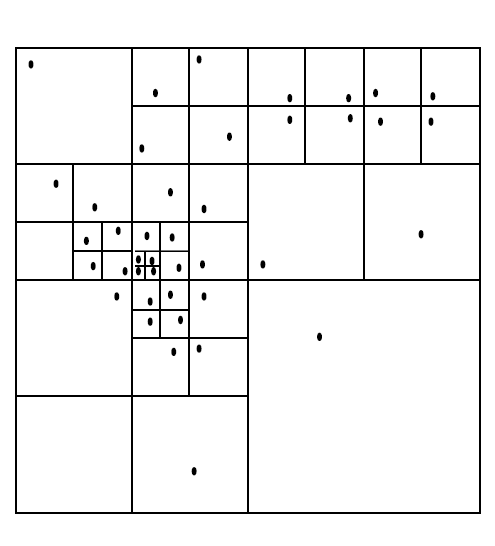
\includegraphics[width=\textwidth]{Theory/Figs/SpatialBarnesHut.png}
        \caption{Spatial domain}
    \end{subfigure}
    ~ 
    \begin{subfigure}[b]{0.4\textwidth}
        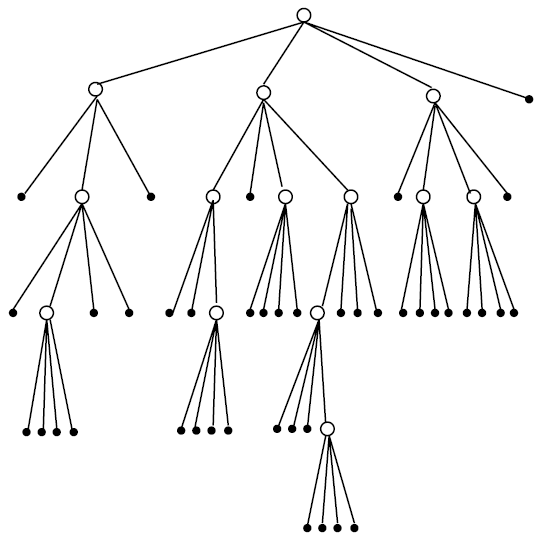
\includegraphics[width=\textwidth]{Theory/Figs/TreelBarnesHut.png}
        \caption{Quadtree representation}
    \end{subfigure}
    \caption{Barnes-Hut recursive subdivision, visualized in 2D for simplicity}
    \label{fig:BarnesHutTree}
\end{figure}


%--------------------------------------------------------%
%----------------------Nomenclature----------------------%
%--------------------------------------------------------%
\nomenclature[z-FMM]{FMM}{Fast Multipole Method}
\nomenclature[z-HLSL]{HLSL}{High-Level Shading Language}
\nomenclature[z-SM]{SM}{Streaming Multiprocessor}
\nomenclature[z-VRAM]{VRAM}{Video Random Access Memory}
\nomenclature[z-DT]{DT}{Distance Transform}
\nomenclature[z-VLIW]{VLIW}{Very Large Instruction Word}
\nomenclature[z-CS]{CS}{Compute Shader}
\nomenclature[z-API]{API}{Application Programming Interface}
%!TEX root = ../thesis.tex

\chapter{Method}

\section{Implementation}
A common application where GPGPU is used is when computing calculation heavy simulations such the N-Body problem described in this thesis. Other common visualizations where GPGPU can be applied is to visualize fractals such as the Julia or Mandelbrot set, named after the french mathematician Gaston Julia and Benoit Mandelbrot. GPGPU has also been used in medicine for accelerated medical image reconstruction \cite{archirapatkave2011gpgpu}, as well as accelerating the Marching Cubes algorithm \cite{johansson2006accelerating}. 

This section describes the implementation of the visualization and the parallel N-Body algorithm in all discussed frameworks, as well as how the measurements were performed and what framework specific features was used. All implementations was implemented in C/C++. The visualization was implemented in the cross-platform API OpenGL on a PC.

\section{Visualization} \label{sec:visualization}

Although not necessary for the evaluation, a visualization of the system was implemented. This was the first step in the implementation process, and the visualization was made using OpenGL. The purpose of the visualization is to make it easier to test and debug the application, which is very difficult without a proper way of visualizing the calculated positions. The N-Body visualization is very similar to a particle system, where each body is represented by a particle. To be able to visualize a very large amount of bodies, the visualization performance is critical, and there are a few ways of implementing a particle system in OpenGL.

The first, and perhaps the most intuitive way is to render a sphere in all positions, by calling \lstinline{glDrawArrays} N times e.g. in a for-loop. This is very inefficient in two regards; a sphere requires a lot of vertices to appear smooth, and drawing a large amount of spheres requires a large amount of vertex data. The second reason this is inefficient is because all SM's (Streaming Multiprocessor) on the GPU will be dedicated to drawing a single polygon, resulting in a huge amount of performance loss. However, since the particles are so small, they don't have to be rendered with a high resolution. A commonly used trick when rendering particle systems is to represent each particle as a quad with a semi-transparent texture with a circle. Each particle will thus only consist of four vertices, which is far less than if each particle was represented by a sphere. The quad is then rotated so that the quad's always faces the camera, giving the illusion that the particle is actually a sphere (or whatever shape the texture represents). This technique is known as \textit{billboarding}.

\nomenclature[z-SM]{SM}{Streaming Multiprocessor}

The solution to the second problem is a bit more complex, and a few solutions exists.
One way is to generate a single vertex buffer object (VBO) with all the particles in them. This is a easy and effective solution that works on all platforms. 

The second way is to use geometry shaders to render a particle in each position. The downside to using geometry shader is that geometry shaders is only supported in systems with OpenGL version 3.2+, and is thus not very portable. 

The third way is to use instancing, meaning that a single mesh is used, but many instances of the mesh. This solution has a nice balance between performance and availability and was thus chosen in this implementation. To achieve this, two main VBO's are used: one VBO containing the positions of the quad, i.e. four vertex coordinates, and a second VBO of size $n$ containing the positions of the instances of the quad, where $n$ is the number of instances. The quad is then rendered using \lstinline{glDrawArraysInstanced(GL_TRIANGLE_STRIP, 0, 4, n)} \cite{OpenCLDocs}, where the first parameter states that the object should be rendered as a triangle strip, i.e. a series of connected triangles, sharing vertices. The second parameter specifies the starting index in the enabled arrays. The third parameter specifies the number of indices to be rendered, and the fourth the number of instances. The quad positions are passed to the vertex shader as an attribute, and the shader then translates the quad into its correct position. The result of the implementation can be seen in figure \ref{fig:OpenGLEarlyVis}, where $n=3.5 \times 10^6$, running at a stable ~60fps on a Nvidia GTX970 GPU. Each quad is rendered in a random $(x,y,z)$ position in a given bounding box.


\begin{figure}[!htpb]
    \centering
    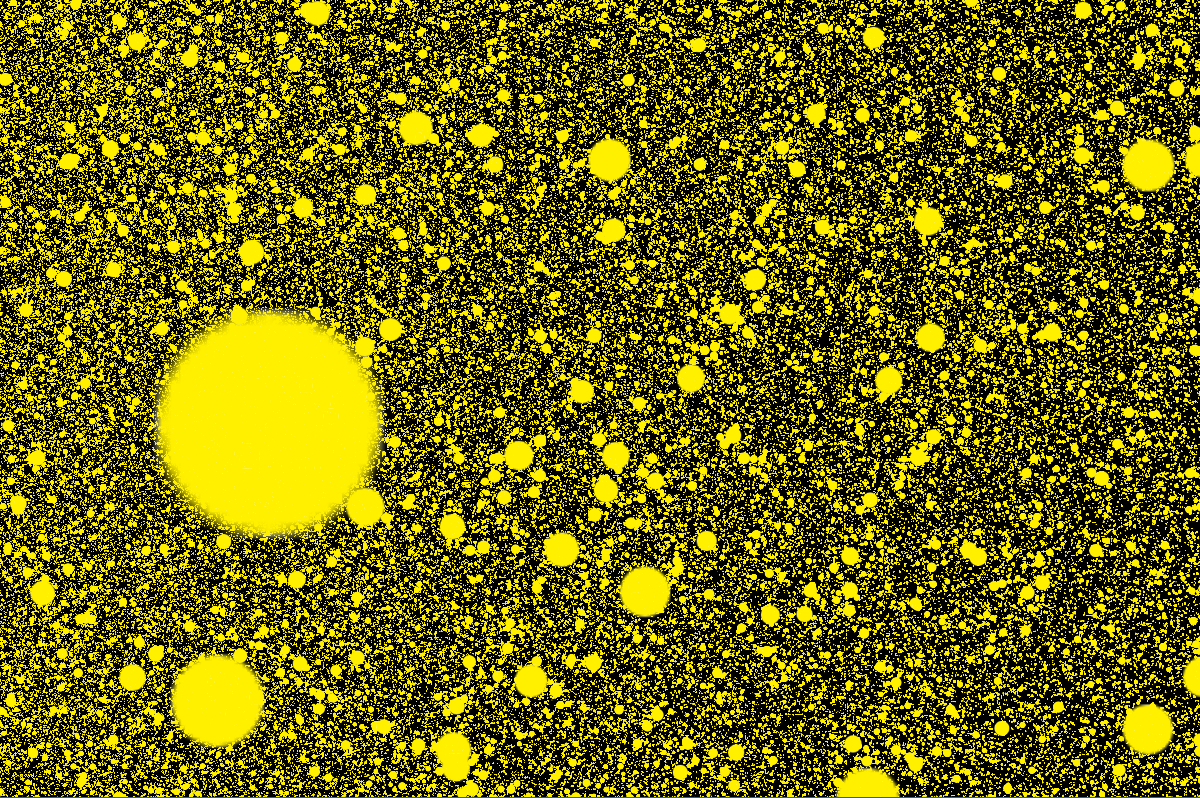
\includegraphics[width=0.8\textwidth]{Method/Figs/OpenGLVis_N=3500000.png}
    \caption{Instanced quad rendering, 3.5*10^6 instances}
    \label{fig:OpenGLEarlyVis}
\end{figure}


\section{Sequential}

This section will describe how a sequential implementation of the all-pairs N-body algorithm was implemented, followed by an optimized sequential implementation using the Barnes-Hut method. \cite{barnes1986hierarchical}


\subsection{All-pairs implementation}
With the particle system visualization implementation described in section \ref{sec:visualization} as a template, a sequential all-pairs N-Body simulation was implemented. A particle is represented by a data structure which contains the position, velocity and mass of the particle. These particles are then instantiated and given a random position. All particles are given the same amount of mass, which makes it easier to analyze the simulation. To make the visualization more visually interesting, the particles are placed in a galaxy like structure using polar coordinates using a random $\varphi$ angle, and a random radius $r$ such that $x = r \ cos \ \varphi, \ y = r \ sin \ \varphi$. If the particles index is even it is translated with a constant length in the positive x-direction, whilst if the index is odd, it is translated in the negative x-direction resulting in two separated galaxy shapes.

To further mimic the behavior of a galaxy, each particle is given a speed according to:
\begin{equation}
    \boldsymbol v = (\boldsymbol c - \boldsymbol p) \times  \boldsymbol z
\end{equation}
\noindent where $\boldsymbol v$ is the velocity of the particle, $\boldsymbol c$ is the center of the galaxy, $\boldsymbol p$ is the position of the particle and $\boldsymbol z$ is the $z$ vector $(0, 0, 1)$. This results in that each particle will spin around the center of the galaxy, simulating how stars in a real galaxy behaves.

Once the system has been initialized, the integration is done in two separate steps. First, the net force $F$ applied on each particle is calculated as it is affected by gravity from all others according to equation \ref{eq:totGravForce}. In a sequential all-pairs implementation, this is typically done by using a nested for-loop resulting in a time complexity of $O(n^2)$. The next step is to update the position of the particle which is done using a first order Euler integration according to:
\begin{equation} \label{eq:EulerIntegrationPosition}
    \boldsymbol p' = \boldsymbol p + F * \Delta t
\end{equation}
\noindent where $p'$ is the new particle position, $p$ is the old position, $F$ is the net force applied to the particle and $\Delta t$ is the delta time of the simulation.
Since this is a first-order method, the error grows quickly with a local error proportional to the square of the step size, and a global error proportional to the step size. The step size of the Euler method used in this simulation does thus depend on the delta time which may vary on different systems. To prevent this a constant $\Delta t = c$ is used, with a small enough constant $c$ so that the integration is accurate enough. This simulation does not aim to be an physical accurate simulation so this integration method works well in this implementation.


\subsection{Octree construction} \label{subsec:OctreeConstruction}
The next step in the implementation was to start working on the Barnes-Hut algorithm by creating an octree from the particles in the particle system. This procedure follows the theory described in section \ref{subsec:BarnesHut} and illustrated in figure \ref{fig:BarnesHutTree}. The octree is represented as a data structure containing the spatial bounds of the cell, the spatial position of the node's center of mass, as well as the total mass contained in the node. It also contains it's eight children, which are of the same kind of data structure, thus resulting in a recursive data structure. The first step to building the tree is to find the bounds of the entire particle system, which is done in a simple reduction algorithm. With this information, the root node of the octree can then be constructed with the given bounds. The next step is to insert the positions of the particles which is done recursively. The position of the particle to be inserted is passed as an parameter, and the tree is then recursively traversed to find the respective node to insert the particle in. If this node is found to be already occupied with another particle, the node is then subdivided into eight new nodes, and the two particles are then moved into their respective new node. 

A problem with the insertion is to know what octant the particle should be inserted to. Since there are eight octant's this can be represented as a single byte. By comparing the position to be inserted with the middle of the cells x,y,z dimensions, this problem is reduced to a single binary expression by following a set of fixed rules. Pseudocode for this procedure can be seen in algorithm \ref{alg:OctreeBuild}, the procedure \lstinline{insert} is called for the root of the tree once for each particle. The resulting octree applied to a system with 2048 particles is visualized in figure \ref{fig:OctreeVisualized}.

Once the tree has been constructed, the next step is to calculate each nodes center of mass (COM) and the total mass contained inside the spatial domain that the node represents. This is again done by utilizing recursion. Each nodes COM is the average of it's children's COM and its total mass is the sum of it's children's total mass. The algorithm starts by calculating the root's COM and total mass, which recursively steps through the tree, calculating the COM of each nodes as it traverses the tree. The termination condition of the recursion is when a leaf node, or a uninitialized empty cell is reached.

\nomenclature[z-COM]{COM}{Center of Mass}

\begin{figure}[!htbp]
    \centering
    \begin{subfigure}[b]{0.65\textwidth}
        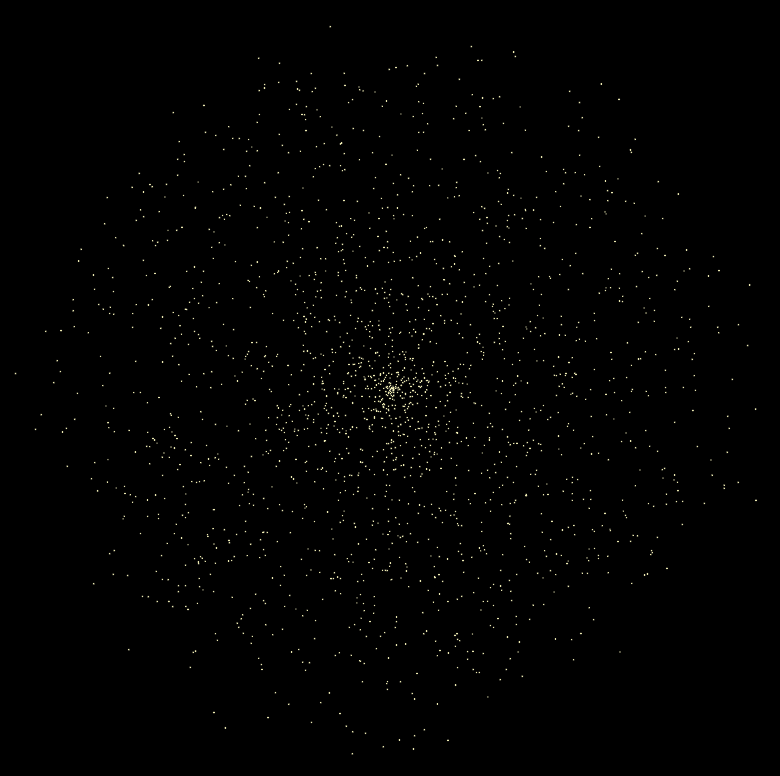
\includegraphics[width=\textwidth]{Method/Figs/PSNoBounds.png}
        \caption{Particle system}
    \end{subfigure}
    ~ 
    \begin{subfigure}[b]{0.65\textwidth}
        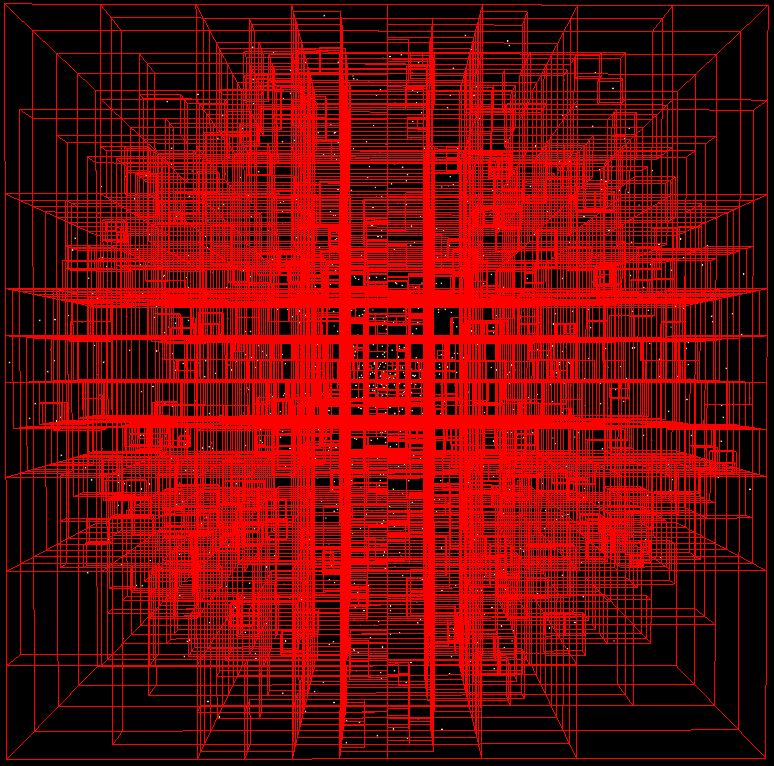
\includegraphics[width=\textwidth]{Method/Figs/PSWithBounds.png}
        \caption{(a) with rendered octree bounds}
    \end{subfigure}
    \caption{Particle system subdivided into an octree}
    \label{fig:OctreeVisualized}
\end{figure}


\begin{algorithm}[!h]
    \caption{Building octree pseudocode}
    \label{alg:OctreeBuild}
    \begin{algorithmic}[1]
    
    \Procedure{Insert}{$x, y, z, data$}
        \If{$node.isEmpty$}
            \Comment{Turn into leaf}
            \State $node.posx := x$
            \State $node.posy := y$
            \State $node.posz := z$
            \State $node.data := data$
        \Else
            \Comment{Node already contains data}
            \If{$node.isChild$}
                \Comment{Subdivide and move into appropriate child}
                \State \Call{InsertSub}{$node.posx, node.posy, node.posz, node.data$}
                \State $node.data = NULL$
            \EndIf
            \State \Call{InsertSub}{x,y,z, data}
        \EndIf
    \EndProcedure
    
    \Procedure{InsertSub}{$x,y,z, data$}
        \State $sub := 0$
        
        \If{$x > midX$}
            \Comment{Children 0,2,4,8 have positive x-coordinates}
            \State $sub += 1$
            \State $newMinX := midX$
            \State $newMaxX := maxX$
        \Else
	        \State $newMinX = minX$
		    \State $newMaxX = midX$
        \EndIf
        
        \If{$y > mid_y$}
            \Comment{Children 0,1,3,4 have positive y-coordinates}
    		\State $sub += 2$
    		\State $newMinY := midY$
    		\State $newMaxY := maxY$
    	\Else
    		\State $newMinY := minY;$
    		\State $newMaxY := midY;$
    	\EndIf
    
    	\If{$z > midZ$}
    	    \Comment{Children 0,1,2,3 have positive z-coordinates}
    		\State $sub += 4$
    		\State $newMinZ := midZ$
    		\State $n_max_z := maxZ$
    	\Else
    		\State $newMinZ := minZ$
    		\State $newMaxZ := midZ$
    	\EndIf
    	
    	
    	\If{!children[sub]}
    	    \Comment{$sub$ will now contain the octant index,  $sub \in {0,8}$}
        	\State \begin{varwidth}[t]{\linewidth}
                $children[sub] := new OctreeNode($ \par
                \hskip\algorithmicindent $newMinX, newMinY, newMinZ,$\par
                \hskip\algorithmicindent $newMaxX, newMaxY, newMaxZ)$
            \end{varwidth}
            
        \EndIf
	    \Call {$children[sub]->insert$}{$x, y, z, usr_data$}
        
    \EndProcedure
        
    \end{algorithmic}
\end{algorithm}    


\subsection{Barnes-Hut force calculation}
Once the tree has been built and the COM of each node has been calculated, the force calculation can begin. Besides the tree, an container containing information about all particles in the systems is used to simplify the data management. Each particle in this container is similar to that of the cells in the tree described in section \ref{subsec:OctreeConstruction}. The particle data structure contains information about the particles mass, position and velocity. This makes the force calculation simpler since the tree can be traversed once for each particle when calculating its net-force, which is a procedure that can easily be parallelized. 

The force calculation for a particle $p$ starts by traversing the tree from the root and then recursively traverses the tree. For each node it traverses, the euclidean distance from the particles position to the COM of the current node is calculated according to: 

\begin{equation} \label{eq:EucDist}
    d(\boldsymbol q, \boldsymbol p) = d(\boldsymbol p, \boldsymbol q) = \sqrt{(p_x-q_z)^2 +(p_y - q_y)^2 + (p_z - q_z)^2}
\end{equation}

\noindent where $q$ and $p$ is the position of the particle and the node. If this distance is equal to zero, it means that the current node is the same node as the particle, and the traversal continues. If the COM of the node is far away enough, the entire sub-tree of the node can be approximated as a single point mass and the force can be calculated using the COM and the mass of the node. If the node is to close to the particle, the sub-tree has to be "opened" and the traversal continues through the sub-tree, recursively calculating the net-force as the tree is traversed. 

One of the problems with the force calculation is what the distance that decides if a node is far away enough so that the sub-tree can be approximated should be. Barnes. et. al. does not mention a general strategy how this distance condition is specified  \cite{barnes1986hierarchical} . Burtscher et. al. uses a constant cutoff distance, which specifies when a node is far away enough \cite{burtscher2011efficient}.
This implementation uses a more general approach to this problem. The average width of the nodes bounds is calculated according to equation \ref{eq:Wavg}, where the max and min variables represent the bounds of the current node. The calculated average width is then used to calculate the ratio between the width and the distance to the node. If this width-to-distance ratio is smaller than a constant $c$, the node is considered to be far away enough to be evaluated as a single point. 

\begin{equation} \label{eq:Wavg}
    \begin{split}
    W_{avg} = &((max_x - min_x) + \\
              &(max_y - min_y) + \\
              &(max_z - min_z)) / 3 \\
    \end{split}
\end{equation}

When the net-force for all particles have been calculated, the position of the node is updated. It is important that this step is done after all of the forces have been calculated to get a correct simulation.
When the forces are calculated, the velocity property of each particle is updated. The position update is then simply done by applying equation \ref{eq:EulerIntegrationPosition} for each particle. With the position update, the simulation step is concluded. The tree is deallocated before beeing rebuilt the next simulation step. 

\section{CUDA} \label{sec:CUDAImplementation}
Once a sequential implementation was in place the work on porting the implementation to CUDA was started.
The octree data structure was built using pointers, pointing to its child sub-trees. This creates two problems when copying the tree structure to the GPU. The first problem is that the size of the tree is unknown and changes very frequently as the tree is rebuilt every simulation step, resulting in an uncertain amount of data to be transferred to the device. Although the size of the tree can be calculated, either when the tree is beeing built, or by a simple depth- or breadth-first traversal of the tree once the tree has been constructed. This solution does however only solve the first problem.

The second problem is that pointers in the octree point to a memory location in the heap memory, which when transferred to the device must be updated to point at the correct position in the VRAM, which would be a performance heavy task. Moreover, complicated structures involving a lot amount of pointers works poorly performance-wise in CUDA, since all the pointer chasing might drastically decrease the total memory bandwidth. 

The solution to both problems is to flatten the tree into an array with a fixed size $n > N$, where $N$ is the number of bodies. The tree will have $N$ leaves, so the size of the array has to have a fixed size which is bigger than the amount of bodies. Implementation wise this was done in two steps.
The first step was to do an iterative breadth-first traversal of the tree, starting from the root, and inserting the traversed nodes into the array, as well as assigning the index to each node. This results in that the array will be sorted top-down, left-right from the tree with the root at index one, visualized on a binary tree in figure \ref{fig:BreadthFirstTreeIndices}. Now that the tree has been flattened into a single list, the child pointers of each node can be replaced with the indices of the child nodes which lies in the same list as the node, making the requirement of pointers in the CUDA kernel redundant and avoiding the the pointer chasing issue.

\begin{figure}[!h]
    \centering
    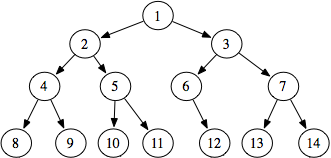
\includegraphics[width=0.6\textwidth]{Method/Figs/breadthFirstTree.png}
    \caption{Order of the flattened tree when a breadth-first flattening algorithm is applied to a binary tree}
    \label{fig:BreadthFirstTreeIndices}
\end{figure}

Now that the octree has been flattened into a tree, it can effortlessly be copied to the device since both the size of the flattened tree is known, and the pointers to each nodes children has been abstracted away and been replaced with indices in the flattened tree, and since CUDA supports the ability of passing class objects to a kernel, the flattened array consisting of octree nodes could simply be passed to the kernel as an argument. 

The remaining part of the algorithm is now reduced to two well parallelizable problems. The first is to calculate the net force of each particle, and the second to update the positions of each particle. The sequential force calculation handles one particle at a time, and traverses the tree once for each particle. This problem is well parallelizable by letting each thread handle one particle. The position update was parallelized in a similar fashion, each thread updates the position of a particle in parallel by using the Euler integration method described in equation \ref{eq:EulerIntegrationPosition}.

The sequential algorithm which was implemented before the CUDA implementation started utilizes recursion to traverse the tree when calculating forces. All Nvidia GPU's of compute capability 2.0 and higher support a stack and can thus utilize recursive functions in CUDA, making the tree traversal in the kernel very similar to the sequential tree traversal. However since recursive calls can't be inlined, and since the amount of overhead spawned when allocating memory for the recursive calls increases, they might significantly decrease the performance due to the spawned overhead when using recursion. Thus an iterative tree-traversal was implemented as well in a breadth-first fashion. The standard and most popular way of doing an iterative breadth-first traversal is by using a queue. All children of the active node is pushed onto the queue, and each iteration the first element in the queue is selected, iteratively pushing each nodes children onto the queue. CUDA does not support the use of the \lstinline{std::queue} in kernel code, so a manual FIFO (First In, First Out) queue data-structure was implemented which was used to implement an iterative tree traversal CUDA kernel.
Since CUDA supports C++ in kernels the queue could be implemented as a datastructure, containing expected member functions such as \lstinline{push(), pop()} etc. To avoid pointer chasing, the queue is implemented using an array as well as integers indexing the front and the back of the queue. The code for the queue can be seen in listing \ref{lst:MyQueue}.




\clearpage
\begin{lstlisting}[caption={Device queue used for iterative traversal of the tree}, label={lst:MyQueue}, frame=single] 

struct MyQueue {
	static const int MAX_SIZE = 10000;
	int f = -1, r = -1;
	int A[MAX_SIZE];

	bool empty() {
		return (f == -1 && r == -1);
	}
	bool isFull() {
		return (r + 1) % MAX_SIZE == f ? true : false;
	}
	void push(int x) {
		if (isFull()) {
			return;
		}
		if (empty()){
			f = r = 0;
		}
		else {
			r = (r + 1) % MAX_SIZE;
		}
		A[r] = x;
	}
	void pop()
	{
		if (empty()) { return; }
		else if (f == r) {
			r = f = -1;
		}
		else {
			f = (f + 1) % MAX_SIZE;
		}
	}
	int front(){
		if (empty()) {
			return -1;
		}
		return A[f];
	}
};
\end{lstlisting}


\section{OpenCL} \label{sec:OpenCLImplementation}

Once the CUDA implementation was done, the work started on the implementation of an OpenCL implementation. To be able to perform a fair comparison between the selected frameworks, the same host program that was used for the CUDA implementation was used for the OpenCL implementation as well. This works well since the main program is implemented in a way so that the device part of the code is well abstracted away from the main application. The host is responsible for building the octree, flattening the octree into an array as well as the graphical simulation, the device part of the code is responsible for calculating forces and updating the positions of the bodies. The device part of the application is separated into its own class object, thus abstracting it away from the main application. 

The OpenCL distribution used in this implementation is Nvidia's OpenCL implementation, version 1.2, which is the newest version developed by Nvidia. 
Although OpenCL are in many aspects very similar to CUDA, some major differences exist. Since OpenCL does not only target GPU devices, but a wider range of parallel hardware (see section \ref{sec:OpenCLTheory}), the implementation needs to specify what device that the parallel kernel should run on. This step is automated by CUDA since it selects the default GPU device available on the system. Since this implementation was performed at a system containing only one GPU, this implementation selects the first available GPU residing in the system. Moreover, unlike CUDA where the device code is processed at compile time using Nvidia's NVCC compiler, OpenCL has to compile the kernel code during runtime. Although the kernel code can be written inline as a string, the common practice is to separate the device and host code which was done in this implementation. The kernels are written in separate \lstinline{.cl} files which is read into a string in the host application, and compiled at run time.

Similar to the CUDA implementation, the parts of the N-Body simulation that has been parallelized is the force calculation as well as the position updating. The flattened tree that is to be copied to the device is a data structure containing a list of class objects, \lstinline{OctreeNode}. To get this data to the device in CUDA is to just do a simple copy of the array to the device memory since CUDA kernels are based on C++ and does thus support classes. Nvidia's OpenCL version 1.2 which is used in this implementation uses the language OpenCL C for device code and does thus not support this feature. Newer versions of OpenCL (v2.0, released in 2013) does support OpenCL C++ in kernels which is based on C++11 and allows for the creation of classes, templates, operator overloading, function overloading etc \cite{OpenCLC++Introduction}. OpenCL C++ does however not support certain C++ features such as exceptions, memory allocation, recursion and function pointers. Although Nvidia is a major backer to OpenCL, Nvidia's latest version of OpenCL is version 1.2, and does thus not support C++ features, so the device code has to be written in OpenCL C. This means that the process of copying the flattened tree to the device is more cumbersome than in the CUDA implementation. Although OpenCL C does not support classes, it supports data structures to be copied between the host and the device. Thus the flattened tree was reworked to contain data structure representations of the \lstinline{OctreeNode} class. This step is done in the host algorithm that flattens the tree. Now that the tree has been flattened and each node is represented as a data structure instead of a class object, the flattened tree can be copied to the device.

As mentioned in section \ref{sec:CUDAImplementation}, all Nvidia GPU's of compute capability 2.0 support recursive calls in kernels, and although the GPU used for the OpenCL implementation is the same as the CUDA implementation and does thus hardware-wise support recursive calls, OpenCL does not. The approach to the kernel implementation is thus different to the CUDA implementation. Since the recursive traversal of the tree is more intuitive and simpler, it was the first force calculation algorithm that was implemented in CUDA, but since OpenCL does not support recursion inside kernels, the iterative version was implemented straight away. To perform a breadth-first tree traversal, the most common iterative way is to used a queue, where non-visited nodes are enqueued. As mentioned in section \ref{sec:CUDAImplementation}, CUDA does not support the std library, which is also the case in OpenCL, and an own implementation of a queue was made. In CUDA this was done using a C++ \lstinline{struct}, containing initialized member variables and member functions expected from a queue such as \lstinline{push(), pop(), front()} and \lstinline{empty()}. However since OpenCL C is based on C99, where data structures can't contain member functions, and structure variables can't be given a default value, the code responsible for pushing, popping etc. from the queue had to be inlined in the kernel.


\section{DirectCompute} \label{sec:DirectComputeImplementation}
Compared to CUDA and OpenCL, DirectX Compute Shaders, or DirectCompute, is very different. Whilst CUDA and OpenCL are frameworks developed with the purpose of GPGPU, DirectCompute is more similar to traditional graphics programming and resembles traditional GPGPU using fragment-/pixel-shaders. DirectX developed by Microsoft, for Microsoft systems, is widely available on Microsoft systems, and DirectX 11 is included in systems running Windows 7 or newer which as of February 2018 is ~96\% of all windows systems, see fig \ref{fig:WindowsStats}. \cite{WindowsStats}


\begin{figure}[!h]
    \centering
    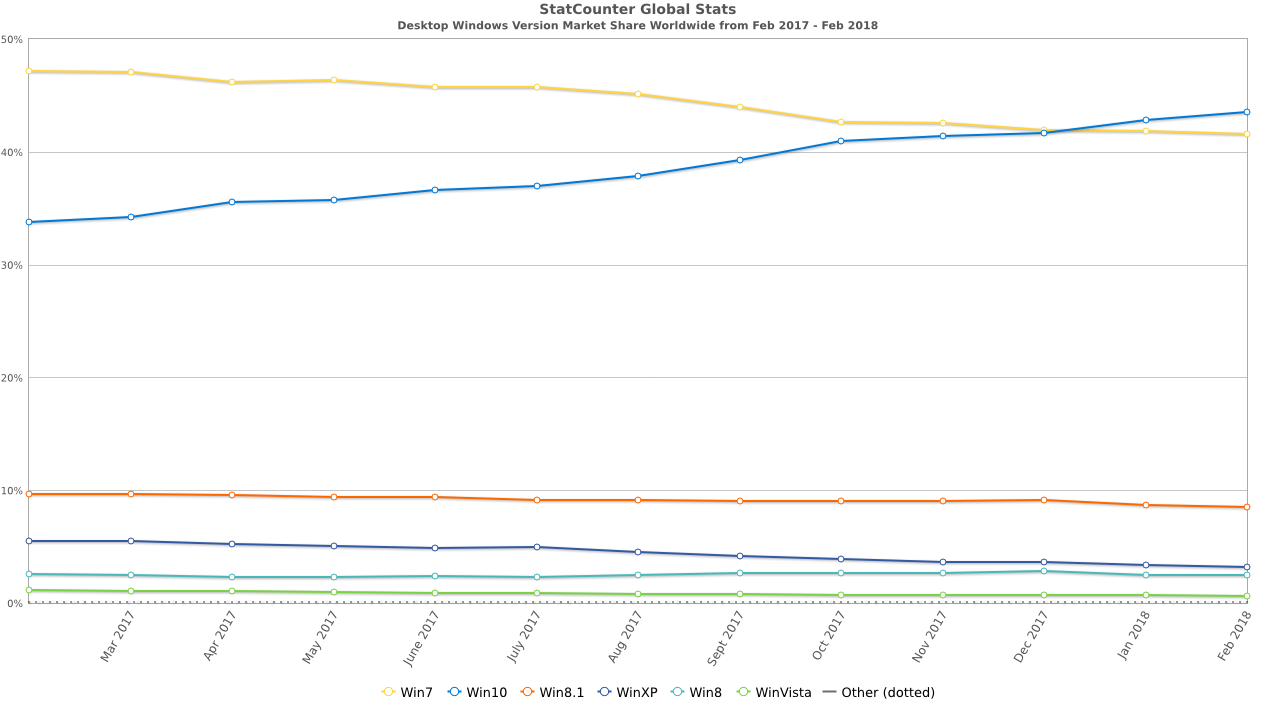
\includegraphics[width=0.8\textwidth]{Method/Figs/StatCounter-windows_version-ww-monthly-201702-201802.png}
    \caption{Desktop Windows Version Market Share Worldwide}
    \label{fig:WindowsStats}
\end{figure}



Released as a part of the Direct3D 11, Microsoft's Compute Shader (CS) is an alternative method of performing general purpose computing on the GPU \cite{Direct3D11Features}. Similar to a CUDA or OpenCL kernel, the CS is similar to a vertex- or pixel-shader but with the purpose of doing more general computing, and is written in High Level Shading Language (HLSL), also developed by Microsoft. 


Compared to CUDA and OpenCL, the initial setup procedure in a Direct Compute application is more complex and a few steps has to be done before the application is ready to perform the computations. 

The first step is to create a device context and to create a target device on which the computation will be performed.
The device is created by calling the method \lstinline{D3D11CreateDevice}, with arguments defining what type of device that should be created. Since DirectCompute is only supported on systems with Direct3D 10 or 11, this must be taken into account when creating the device. To specify this, a \lstinline{D3D_FEATURE_LEVEL} variable is passed as an argument to the device creation method which specifies which feature levels the device will use. Once the method has been called, the resulting feature level of the device can be determined. This information is important because if the resulting feature level is to low, lower than 10.0, CS is not supported. This method also allows the option to select what hardware the device is referring to, in this implementation the default graphics card is selected.

The second step is to compile the actual HLSL compute shaders. The DirectX provides a method for doing this depending on the DirectX version is running on the system. One thing to keep in mind when creating the CS is what CS shader profile to use. Although there's not much feature-wise difference between CS 4.0 and 5.0, if the system is running Direct3D (D3D) feature level of 11 we generally want to use CS 5.0 as it allows for better performance on 11-class hardware. The HLSL CS source file can then be compiled by using either \lstinline{D3DCompileFromFile} or \lstinline{D3DX11CompileFromFile}, depending on the feature level of the hardware. If the source file is successfully compiled, a CS instance object can then be created by from the compiled shader code.

The process of performing the computation on the device is similar to the process in CUDA and OpenCL. First memory has to be allocated on the device. Similar to graphics programming, DirectCompute uses buffers to achieve this. These buffers have a wide variety of options which are set by using a \lstinline{D3D11_BUFFER_DESC} data structure instance, passed as an argument when creating the buffer. This description may contain information such as if it is a constant buffer, if it is a raw or structured buffer, the size of an element in the buffer as well as the total size of the buffer. This data structure along with the data the buffer will contain is then be passed to \lstinline{ID3D11Device::CreateBuffer} which creates an buffer instance object. 

Before the CS can be launched, view interfaces has to be generated from the buffers which can then be passed accessed by the CS. Two types of view interfaces was used in this implementation: \lstinline{ID3D11ShaderResourceView} and \lstinline{ID3D11UnorderedAccessView}, where the main difference is the CS has read-only access to a a shader resource view (SRV), whilst the CS has read-and-write access to a unordered access view (UAV) at the cost of performance, UAVs does thus act as outputs from the compute shader and is the only type of view interface that can be used as an output buffer. Constant buffers can be passed straight to the shader without requiring the use of SRVs or UAVs.

Now all information needed to launch the CS is received. Although it requires a lot of code to set up buffers and view interfaces, the process of launching a CS is trivial. Similar to graphics programming, we first have to bind the shader to make it active, this is done by using the method \lstinline{CSSetShader} with the corresponding CS instance as an argument. We can then pass the view interfaces and constant buffers to the CS in a similar fashion by calling \lstinline{CSSetUnorderedAccessViews}, \lstinline{CSSetShaderResources} or \lstinline{CSSetConstantBuffers}. The CS is then launched by calling \lstinline{Dispatch(X,Y,Z)}, where \lstinline{X,Y,Z} specifies the number of thread groups to be launched in each dimension. The number of thread groups (blocks in CUDA, work groups in OpenCL) is thus specified from the host when dispatching the CS, the number of threads per group is specified on the device in the CS by using the \lstinline{numthreads(X,Y,Z)} attribute, which specifies how many threads should be dispatched in each thread group. E.g a \lstinline{Dispatch(8,1,1)} with a \lstinline{numthreads(512,1,1)} would dispatch a compute shader with a total of 8 thread groups, each group containing 512 threads, thus the total number of threads would be 4096. The thread and group index can then be retrieved with the keywords listed in table \ref{tab:HLSLIndexKeywords}.
The result from the CS can then be retrieved by using the method \lstinline{Map}, and copy the data back into its original container with a \lstinline{memcpy}. 

\begin{table}
    \begin{tabularx}{\textwidth}{ |X|X| }
      \hline
      \rowcolor{gray}
      \textbf{Variable name}    & \textbf{Description}  \\ \hline                         
      SV\_GroupIndex            & Flattened 1D index of a thread within a thread group \\ \hline
      SV\_DispatchThreadID      & Global thread index, sum of SV\_GroupID * numthreads and GroupThreadID            \\ \hline
      SV\_GroupThreadID         & 3D Indices for a thread within a group \\ \hline
      SV\_GroupID               & Indices for which thread group a compute shader is executing in \\ \hline
    \end{tabularx}
\caption{\label{tab:HLSLIndexKeywords} HLSL index variables.}
\end{table}

Since all data that is to be passed to the CS has to be bound to a buffer, there is no way of directly passing single data elements such as integers or floating points. The common practice of achieving this is to create a data structure containing all single element variables, and then generate a single element constant buffer with the data structure which is passed to the CS. Since it is a constant buffer, this buffer can be passed to the CS without the need of a SRV or UAV.

The UAVs, SRVs and constant buffers are unlike OpenCL and CUDA not recieved as arguments to the kernel function, but as "global" variables inside the shader code. The buffer is recieved according to \lstinline{bufferType<T> bufferName : register(Type#)} in the hlsl code, where the \lstinline{#} specifies in what register slot the buffer is assigned, which is specified when setting the buffer from the host, and the \lstinline{Type} is a single character describing the register type. Although many types of HLSL buffers exists, the ones used in this implementation are listed in table \ref{tab:HLSLBufferTypes}. The register types used in this implementation are listed in table \ref{tab:HLSLRegTypes}.


\begin{table}
    \begin{tabularx}{\textwidth}{ |X|X| }
      \hline
      \rowcolor{gray}
      \textbf{Buffertype}   & \textbf{Description}  \\ \hline 
      cbuffer               & Constant buffer       \\ \hline
      RWBuffer              & Raw buffer            \\ \hline
      RWStructuredBuffer    & Raw structured buffer \\ \hline
    \end{tabularx}
\caption{\label{tab:HLSLBufferTypes} HLSL buffer types.}
\end{table}

\begin{table}
    \begin{tabularx}{\textwidth}{ |X|X| }
      \hline
      \rowcolor{gray}
      \textbf{Register type}   & \textbf{Description}  \\ \hline 
      b & Constant buffer               \\ \hline
      t & Texture and texture buffer    \\ \hline
      c & Buffer offset                 \\ \hline
      s & Sampler                       \\ \hline
      u & Unordered Access View         \\ \hline
    \end{tabularx}
\caption{\label{tab:HLSLRegTypes} HLSL register types.}
\end{table}



Similar to the CUDA and OpenCL implementation, there are three datastructures that has to be passed to the CS in order to calculate the forces and update the positions:

\begin{itemize}
    \item The positions of the particles 
    \item A container containing more information about each particle such as it's velocity and mass 
    \item The flattened octree. 
\end{itemize}

Both the position container and the particle container has to be updated in the CS, and these are thus passed to the shader as UAVs. The flattened octree container however is unmodified in the shader and can thus be passed as a SRV to the shader for optimization purposes. To minimize the amount of overhead generated by copying data between the host and the device, the shader views are copied once before the force calculation CS is dispatched. There is no need to retrieve the result from this dispatch since the required data for the position update CS is already on the device. Once both dispatches has been finished, the data can be copied back into it's original containers.

\vskip .5em
Two types of CS was used in the implementation, one CS responsible for calculating the forces applied on each body in the system, and a second CS responsible for updating the positions. Since the positions have to be updated after the force calculation has been finished for each simulation step, two CS dispatches was made to be able to synchronize between the thread groups. 

The first CS, the force calculation CS, was ported from the OpenCL force calculation kernel and is very similar. 
The CS responsible for updating the positions of the bodies is very trivial. Since the force calculation has been done before this shader is dispatched, all information needed to calculate the new position of the body is obtained. The position is updated by moving its position in the direction of its velocity vector, calculated in the force update CS, times the delta time. Since the positions have to be retrieved and read by the host to later be passed to the visualization, the position vector is converted into a raw buffer, and passed to the shader as an UAV. 

The force calculation CS is more complex than the position update CS. Since HLSL does not support recursive calls, an iterative implementation using a queue was implemented. Although shader model 5.0 used in this implementation support C++ like data structures and classes with member functions and variables, some limitations exists. HLSL classes/data structure cannot contain member variables with initial values. This can however easily be avoided by e.g using a initialize member function. However when using a data structure method inside a loop, the loop is forced to be unrolled. When performing the iterative tree traversal using a queue, a while-loop is running until the queue is empty. The problem is that the while loop cannot be unrolled, and thus it's not a viable solution to use a data structure representing a queue. The solution to this was similar to how the same problem was solved in the OpenCL implementation as described in section \ref{sec:OpenCLImplementation}, by in-lining the push/pop operations inside the CS. The actual force calculation is very similar to the force calculation described in section \ref{sec:CUDAImplementation} and \ref{sec:OpenCLImplementation}.


\section{SkePU}






\nomenclature[z-SRV]{SRV}{Shader Resource View}
\nomenclature[z-UAV]{UAV}{Unordered Access View}
\nomenclature[z-VBO]{VBO}{Vertex Buffer Object}
\nomenclature[z-D3D]{D3D}{Direct3D}
\nomenclature[z-FIFO]{FIFO}{First in, first out}
\nomenclature[z-HLSL]{HLSL}{High Level Shading Language}
%!TEX root = ../thesis.tex

\chapter{Results}


%!TEX root = ../thesis.tex

\chapter{Discussion}


%!TEX root = ../thesis.tex

\chapter{Conclusion}




% ********************************** Back Matter *******************************
% Backmatter should be commented out, if you are using appendices after References
%\backmatter

% ********************************** Bibliography ******************************
\begin{spacing}{0.9}

% To use the conventional natbib style referencing
% Bibliography style previews: http://nodonn.tipido.net/bibstyle.php
% Reference styles: http://sites.stat.psu.edu/~surajit/present/bib.htm

%\bibliographystyle{apalike}
%\bibliographystyle{unsrt} % Use for unsorted references  
\bibliographystyle{plainnat} % use this to have URLs listed in References
\cleardoublepage
\bibliography{References/references} % Path to your References.bib file


% If you would like to use BibLaTeX for your references, pass `custombib' as
% an option in the document class. The location of 'reference.bib' should be
% specified in the preamble.tex file in the custombib section.
% Comment out the lines related to natbib above and uncomment the following line.

%\printbibliography[heading=bibintoc, title={References}]


\end{spacing}

% ********************************** Appendices ********************************

\begin{appendices} % Using appendices environment for more functunality

%!TEX root = ../thesis.tex
% ******************************* Thesis Appendix A ****************************
\chapter{CUDA Vector Addition} \label{appendix:CUDAVecAdd}
\lstset{language=C++,
                keywordstyle=\color{blue},
                stringstyle=\color{BurntOrange},
                commentstyle=\color{OliveGreen},
                basicstyle=\footnotesize,
                numbers=left,
                stepnumber=1,
                tabsize=4,
}


\begin{lstlisting}
#pragma once
#include "cuda_runtime.h"
#include "device_launch_parameters.h"
#include <stdio.h>
#include <iostream>

const unsigned int SIZE = 1024;

// addition kernel
__global__ void add(const int *in_a, const int *in_b, int *out)
{
	int idx = blockDim.x * blockIdx.x + threadIdx.x;
	if (idx < SIZE)
		out[idx] = in_a[idx] + in_b[idx];
}

int main(){

	// Host pointers for io data
	int *a = new int[SIZE];
	int *b = new int[SIZE];
	int *c = new int[SIZE];

	// Device pointers
	int *d_a, *d_b, *d_c;

	for (int i = 0; i < SIZE; i++){
		a[i] = i;
		b[i] = 2*i;
	}

	// Allocate memory on the device
	const unsigned int size = SIZE * sizeof(int);
	cudaMalloc((void**)&d_a, size);
	cudaMalloc((void**)&d_b, size);
	cudaMalloc((void**)&d_c, size);
	
	// Copy the input data to the device
	cudaMemcpy(d_a, a, size, cudaMemcpyHostToDevice);
	cudaMemcpy(d_b, b, size, cudaMemcpyHostToDevice);

	dim3 dimGrid(1);
	dim3 dimBlock(SIZE);

	// Launch kernel with the given grid and block dimensions
	add <<<dimGrid, dimBlock >>> (d_a, d_b, d_c);

	// Retrieve the result
	cudaMemcpy(c, d_c, size, cudaMemcpyDeviceToHost);

	// Assert that the result is correct
	for (int i = 0; i < SIZE; i++){
		if (a[i] + b[i] != c[i])
			return 1;
	}
	std::cout << "Sucess!" << std::endl;

	// Clean up
	cudaFree(d_a); cudaFree(d_b); cudaFree(d_c);
	delete[] a; delete[] b; delete[] c;

	return 0;
}
\end{lstlisting}
%!TEX root = ../thesis.tex
% ******************************* Thesis Appendix B ********************************

\chapter{Installing the CUED class file}

\LaTeX.cls files can be accessed system-wide when they are placed in the
<texmf>/tex/latex directory, where <texmf> is the root directory of the user’s \TeX installation. On systems that have a local texmf tree (<texmflocal>), which
may be named ``texmf-local'' or ``localtexmf'', it may be advisable to install packages in <texmflocal>, rather than <texmf> as the contents of the former, unlike that of the latter, are preserved after the \LaTeX system is reinstalled and/or upgraded.

It is recommended that the user create a subdirectory <texmf>/tex/latex/CUED for all CUED related \LaTeX class and package files. On some \LaTeX systems, the directory look-up tables will need to be refreshed after making additions or deletions to the system files. For \TeX Live systems this is accomplished via executing ``texhash'' as root. MIK\TeX users can run ``initexmf -u'' to accomplish the same thing.

Users not willing or able to install the files system-wide can install them in their personal directories, but will then have to provide the path (full or relative) in addition to the filename when referring to them in \LaTeX.

\end{appendices}

% *************************************** Index ********************************
\printthesisindex % If index is present

\end{document}
